\documentclass{patmorin}
\listfiles
\usepackage[T1]{fontenc}
\usepackage[utf8]{inputenc}
\usepackage{amsmath}
\usepackage{amsfonts}
\usepackage{amsthm}
\usepackage{graphicx}
\usepackage{enumerate}
\usepackage{amsfonts}
\usepackage{amsthm,mathtools}
\usepackage{pat}
\usepackage{paralist}
\usepackage{stmaryrd}
\usepackage{thm-restate}
\usepackage[usenames,dvipsnames,svgnames,table]{xcolor}

\newcommand{\arXiv}[1]{arXiv:\,\href{https://arxiv.org/abs/#1}{#1}}
%\newcommand{\doi}[1]{\href{https://doi.org/#1}{\tt https://doi.org/#1}}

\usepackage[longnamesfirst,numbers,sort&compress]{natbib}
\usepackage[noabbrev,capitalise]{cleveref}


%\usepackage{doi} % To make plainnat handle doi's properly

% \usepackage[mathlines]{lineno}
% \setlength{\linenumbersep}{2em}
% \linenumbers
% \rightlinenumbers
% \linenumbers
% \newcommand*\patchAmsMathEnvironmentForLineno[1]{%
%  \expandafter\let\csname old#1\expandafter\endcsname\csname #1\endcsname
%  \expandafter\let\csname oldend#1\expandafter\endcsname\csname end#1\endcsname
%  \renewenvironment{#1}%
%     {\linenomath\csname old#1\endcsname}%
%     {\csname oldend#1\endcsname\endlinenomath}}%
% \newcommand*\patchBothAmsMathEnvironmentsForLineno[1]{%
%  \patchAmsMathEnvironmentForLineno{#1}%
%  \patchAmsMathEnvironmentForLineno{#1*}}%
% \AtBeginDocument{%
% \patchBothAmsMathEnvironmentsForLineno{equation}%
% \patchBothAmsMathEnvironmentsForLineno{align}%
% \patchBothAmsMathEnvironmentsForLineno{flalign}%
% \patchBothAmsMathEnvironmentsForLineno{alignat}%
% \patchBothAmsMathEnvironmentsForLineno{gather}%
% \patchBothAmsMathEnvironmentsForLineno{multline}%
% }
%
%
% \allowdisplaybreaks
%\sloppy
%%%%%%%%%%
 \makeatletter
 \def\NAT@spacechar{~}
 \makeatother

\newcommand{\snote}[1]{{\color{red}#1}}

\newcommand{\defin}[1]{\textcolor{Maroon}{\emph{#1}}}

\crefname{lem}{Lemma}{Lemmas}
\crefname{thm}{Theorem}{Theorems}
\crefname{cor}{Corollary}{Corollaries}
\crefname{conj}{Conjecture}{Conjectures}
\crefname{obs}{Observation}{Observations}
\crefname{prop}{Proposition}{Propositions}
\crefname{clm}{Claim}{Claims}
\crefname{openproblem}{Open Problem}{Open Problems}
\crefformat{equation}{(#2#1#3)}
\Crefformat{equation}{Equation #2(#1)#3}

\newcommand{\note}[2]{\noindent{\color{red}[#1:~#2]}}
\newcommand{\notex}[2]{}
\newcommand{\referee}[2]{\noindent\textcolor{blue}{\framebox{\begin{minipage}{\textwidth} Ref \#{#1}: #2\end{minipage}}}}

\DeclareMathOperator{\dist}{dist}
\DeclareMathOperator{\depth}{depth}
\DeclareMathOperator{\ff}{f}
\DeclareMathOperator{\tw}{tw}
\DeclareMathOperator{\pw}{pw}
\DeclareMathOperator{\qn}{qn}
\DeclarePairedDelimiter{\ceil}{\lceil}{\rceil}
\DeclarePairedDelimiter{\floor}{\lfloor}{\rfloor}

\newcommand{\PRlabel}[1]{\label{PR:#1}}
\newcommand{\PRref}[1]{(PR\ref{PR:#1})}

\newcommand{\jlabel}[1]{\label{j:#1}}
\newcommand{\jref}[1]{(J\ref{j:#1})}

\newcommand{\tlabel}[1]{\label{t:#1}}
\newcommand{\tref}[1]{(T\ref{t:#1})}
\newcommand{\ylabel}[1]{\label{y:#1}}
\newcommand{\yref}[1]{(Y\ref{y:#1})}

% \newcommand{\PP}{\mathcal{P}}
\renewcommand{\SS}{\mathcal{S}}

\renewcommand{\ge}{\geqslant}
\renewcommand{\le}{\leqslant}
\renewcommand{\geq}{\geqslant}
\renewcommand{\leq}{\leqslant}

\title{\MakeUppercase{Graph Product Structure for Non-Minor-Closed Classes}}

\author{Vida Dujmovi\'c%
        \thanks{School of Computer Science and Electrical Engineering,
                University of Ottawa, Ottawa, Canada (\texttt{vida.dujmovic@uottawa.ca}).
                Research supported by NSERC and the Ontario Ministry of Research and Innovation.},\,\,
        Pat Morin%
        \thanks{School of Computer Science, Carleton University, Ottawa, Canada (\texttt{morin@scs.carleton.ca}). Research  supported by NSERC and the Ontario Ministry of Research and Innovation.},\,\, and
        David R. Wood\thanks{School of Mathematics, Monash University, Melbourne, Australia (\texttt{david.wood@monash.edu}). Research supported by the Australian Research Council.}
}

\begin{document}
\begin{titlepage}
\maketitle

\begin{abstract}
Dujmovi\'c~et~al.~[\emph{J.~ACM}~'20] recently proved that every planar graph is isomorphic to a subgraph of the strong product of a graph of bounded treewidth and a path. Analogous results were obtained for graphs of bounded Euler genus or apex-minor-free graphs. These tools have been used to solve longstanding problems on queue layouts, non-repetitive colouring, $p$-centered colouring, and adjacency labelling. This paper proves analogous product structure theorems for various non-minor-closed classes. One noteable example is $k$-planar graphs (those with a drawing in the plane in which each edge is involved in at most $k$ crossings). We prove that every $k$-planar graph is isomorphic to a subgraph of the strong product of a graph of treewidth $O(k^5)$ and a path. This is the first result of this type for a non-minor-closed class of graphs. It implies, amongst other results, that $k$-planar graphs have non-repetitive chromatic number upper-bounded by a function of $k$. All these results generalise for drawings of graphs on arbitrary surfaces. In fact, we work in a much more general setting based on so-called shortcut systems that are of independent interest. This leads to analogous results for certain types of map graphs, string graphs, graph powers, and nearest neighbour graphs.
\end{abstract}
\end{titlepage}
\pagenumbering{roman}
\tableofcontents
\newpage

\pagenumbering{arabic}
% \setcounter{\page}{1}
\section{Introduction}
\label{Introduction}

The starting point for this work is the following `product structure theorem' for planar graphs\footnote{In this paper, all graphs are finite and undirected. Unless specifically mentioned otherwise, all graphs are also simple. For any graph $G$ and any set $S$ (typically $S\subseteq V(G)$), let $G[S]$  denote the graph with vertex set $V(G)\cap S$ and edge set $\{uv\in E(G) : u,v\in S\}$.  We use $G-S$ as a shorthand for $G[V(G)\setminus S]$. We use $G'\subseteq G$ to denote subgraph containment; that is, $V(G')\subseteq V(G)$ and $E(G')\subseteq E(G)$.  We say that a graph $G$ is \defin{contained in} a graph $X$ if $G$ is isomorphic to a subgraph of $X$. Undefined terms are in \citep{Diestel5}.} by \citet{DJMMUW20} (improved by \citet{UWY}).

\begin{thm}[\citep{DJMMUW20,UWY}]
	\label{PlanarProduct}
	Every planar graph is contained in: 
	%a subgraph of:
	\begin{compactenum}[(a)]
		\item $H\boxtimes P$ for some graph $H$ of treewidth at most $8$ and for some path $P$,
		\item $H\boxtimes P \boxtimes K_3$ for some graph $H$ of treewidth at most $3$ and for some path $P$.
	\end{compactenum}
\end{thm}

% \note{DW}{In 	\cref{PlanarProduct} and elsewhere, we really should write, ``Every planar graph is isomorphic to a subgraph of''. One alternative is to define that $H$ is \defin{contained} in $G$ if $H$ is isomorphic to a subgraph of $G$. I suggest the latter.}

 \note{DW}{replace $8$ by $6$ and update elsewhere}

Here $\boxtimes$ is the strong product,\!\footnote{The \emph{strong product} of graphs $A$ and $B$, denoted by $A\boxtimes B$, is the graph with vertex set $V(A)\times V(B)$, where distinct vertices $(v,x),(w,y)\in V(A)\times V(B)$ are adjacent if
	$v=w$ and $xy\in E(B)$, or
	$x=y$ and $vw\in E(A)$, or
	$vw\in E(A)$ and $xy\in E(B)$.}
and treewidth\footnote{For a tree $T$, a \defin{$T$-decomposition} of a graph $G$ is a collection $\mathcal{T}=(B_x:x\in V(T))$ of subsets of $V(G)$ indexed by the nodes of $T$ such that
(i) for every $vw\in E(G)$, there exists some node $x\in V(T)$ with $v,w\in B_x$; and
(ii) for every $v\in V(G)$, the induced subgraph $T[v] := T[\{x: v\in B_x\}]$ is connected. The \defin{width} of $\mathcal{T}$ is $\max\{|B_x|:x\in V(T)\}-1$.  A \defin{tree-decomposition} is a $T$-decomposition for any tree $T$. The \defin{treewidth} $\tw(G)$ of a graph $G$ is the minimum width of a tree-decomposition of $G$.  Treewidth is the standard measure of how similar a graph is to a tree. Indeed, a connected graph has treewidth 1 if and only if it is a tree. Treewidth is of fundamental importance in structural and algorithmic graph theory; see \citep{Reed03,HW17,Bodlaender-TCS98} for surveys.} is an invariant that measures how `tree-like' a given graph is; see \cref{ProductExample} for an example. Loosely speaking, \cref{PlanarProduct} says that every planar graph is contained in the product of a tree-like graph and a path. This enables combinatorial results for graphs of bounded treewidth to be generalised for planar graphs (with different constants).

\begin{figure}[!h]
\centering
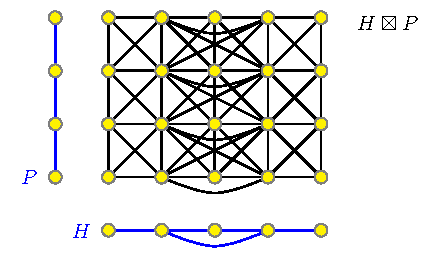
\includegraphics{ProductExample}
\caption{Example of a strong product.
\label{ProductExample}}
\end{figure}

\noindent\cref{PlanarProduct} has been the key tool in solving the following well-known open problems:
\begin{compactitem}
\item \citet{DJMMUW20} use it to prove that planar graphs have bounded queue-number (resolving a conjecture of \citet{HLR92}).
\item  \citet{dujmovic.esperet.ea:planar} use it to prove that planar graphs have bounded non-repetitive chromatic number (resolving a conjecture of \citet{AGHR-RSA02}).
\item \citet{DFMS21} use it to make dramatic improvements to the best known bounds for $p$-centered colourings of planar graphs.
\item \citet{bonamy.gavoille.ea:shorter} use it to find shorter adjacency labellings of planar graphs (improving on a sequence of results starting with the work of \citet{kannan.naor.ea:implicit-stoc,kannan.naor.ea:implicit}). \citet{DEJGMM21} have since used it to find asymptotically optimal adjacency labellings of planar graphs.
\item The result of \citet{DEJGMM21} implies that, for every integer
$n>0$, there is a `induced-universal' graph $U_n$ with $n^{1+o(1)}$ vertices such that every $n$-vertex planar graph is an induced
subgraph of $U_n$. This has recently been extended by \citet{EJM}, who show the existence of a `subgraph-universal' graph with $(1+\epsilon)n$ vertices that contains every $n$-vertex planar graph as a subgraph as well as the existence of an `induced universal' graph with $n^{1+o(1)}$ vertices \emph{and} edges.  The former result is the first progress on subgraph-universal graphs for planar graphs since the $O(n^{3/2})$-vertex construction of \citet{babai.chung.ea:on}.
% aking the first progress on this problem since the work of \citet{babai.xx} in 1984.
\end{compactitem}

% \note{DW}{Delete `from 1992' and  `from 2007'? replace ``going back to 1988~\citep{kannan.naor.ea:implicit-stoc,kannan.naor.ea:implicit}'' by
	% ``starting with the work of \citet{kannan.naor.ea:implicit}''}
% \note{PM}{Was this a referee request, or just because we don't need to sell it anymore?  I'm fine with the change either way, but didn't implement it.}

% \note{DW}{Add \citep{EJM} to the story.}

All of these results hold for any graph class that has a product structure theorem analogous to \cref{PlanarProduct}; that is, for any graph class  $\mathcal{G}$ where every graph in $\mathcal{G}$ is contained in $H\boxtimes P\boxtimes K_\ell$ where $H$ has bounded treewidth, $P$ is a path, and $\ell$ is bounded.\footnote{It is easily seen that $\tw(H\boxtimes K_\ell) \leq (\tw(H)+1)\ell-1$, so we may assume that $\ell=1$ in this definition.} These applications motivate finding product structure theorems for other graph classes. \citet{DJMMUW20} prove product structure theorems for graphs of bounded Euler genus\footnote{The \textit{Euler genus} of the orientable surface with $h$ handles is $2h$. The \textit{Euler genus} of the non-orientable surface with $c$ cross-caps is $c$. The \textit{Euler genus} of a graph $G$ is the minimum integer $g$ such that $G$ embeds in a surface of Euler genus $g$. Of course, a graph is planar if and only if it has Euler genus 0; see \citep{mohar.thomassen:graphs} for more about graph embeddings in surfaces.} and for apex-minor-free graphs\footnote{A graph $M$ is a \textit{minor} of a graph $G$ if a graph isomorphic to $M$ can be obtained from a subgraph of $G$ by contracting edges. A class $\mathcal{G}$ of graphs is \defin{minor-closed} if for every graph $G\in\mathcal{G}$, every minor of $G$ is in $\mathcal{G}$. A minor-closed class is \defin{proper} if it is not the class of all graphs. For example, for fixed $g\geq 0$, the class of graphs with Euler genus at most $g$ is a proper minor-closed class. A graph $G$ is $t$-apex if it contains a set $A$ of at most $t$ vertices such that $G-A$ is planar. A 1-apex graph is \defin{apex}.  A minor-closed class $\mathcal{G}$ is apex-minor-free if some apex graph is not in $\mathcal{G}$.}, and \citet{DEMWW22} do so for graphs in any minor-closed class and with bounded maximum degree. See \cref{Generalisations} for more precise statements and see \citep{DHJLW21} for a survey on this topic.

The main purpose of this paper is to prove product structure theorems for several non-minor-closed classes of interest. Our results are the first of this type for non-minor-closed classes.

\subsection{$k$-Planar Graphs}

We start with the example of $k$-planar graphs. A graph is \defin{$k$-planar} if it has a drawing in the plane in which each edge is involved in at most $k$ crossings, where no three edges cross at a single point (see \cref{sec-k-planar} for a formal definition). Such graphs provide a natural generalisation of planar graphs, and are important in graph drawing research; see the recent bibliography on 1-planar graphs and the 140 references therein \citep{kobourov.liotta.ea:annotated}. It is well-known that the family of $k$-planar graphs is not minor-closed.  Indeed, 1-planar graphs may contain arbitrarily large complete graph minors~\citep{dujmovic.eppstein.ea:structure}. Hence the above results are not applicable for  $k$-planar graphs. We extend \cref{PlanarProduct} as follows.

\begin{thm}
\label{kPlanarProduct}
Every $k$-planar graph is a subgraph of $H\boxtimes P\boxtimes K_{18k^2+48k+30}$, for some graph $H$ of treewidth $\binom{k+4}{3}-1$ and for some path $P$.
\end{thm}

This theorem has applications in diverse areas, including queue layouts  \citep{DJMMUW20}, non-repetitive colouring  \citep{dujmovic.esperet.ea:planar}, $p$-centered colouring  \citep{DFMS21}, and adjacency labelling \citep{DEJGMM21}, which we explore in \cref{Applications}. For example, we prove that $k$-planar graphs have bounded non-repetitive chromatic number (for fixed $k$). Prior to the recent work of \citet{dujmovic.esperet.ea:planar}, it was even open whether planar graphs have bounded non-repetitive chromatic number.

\referee{1}{3. pages 2 – 4: The paragraph following Theorem 2 and Section 1.3
(except for the fact that the apex assumption is necessary) is repetition
of things discussed earlier on in the introduction.}

\note{PM}{Kind of, but I suggest we keep that paragraph and section anyway. Justification: They're both short and they describe the exact bounds for bounded genus graphs, which you don't get from the one-paragraph description in Section~1.0.}

\subsection{Shortcut Systems}

Although $k$-planar graphs are the most high-profile target for a generalization of \cref{PlanarProduct}, we actually prove a substantially stronger result than \cref{kPlanarProduct} using the following definition. A non-empty set $\SS$ of non-trivial paths in a graph $G$ is a \defin{$(k,d)$-shortcut system} (for $G$) if:

\begin{compactitem}
\item every path in $\SS$ has length at most $k$,\footnote{A path of length $k$ consists of $k$ edges and $k+1$ vertices.  A path is \defin{trivial} if it has length 0 and \defin{non-trivial} otherwise.} and
\item for every $v\in V(G)$, the number of paths in $\SS$ that use $v$ as an internal vertex is at most $d$.
\end{compactitem}
Each path $P\in\SS$ is called a \defin{shortcut}; if $P$ has endpoints $v$ and $w$ then it is a \defin{$vw$-shortcut}. Given a graph $G$ and a $(k,d)$-shortcut system $\SS$ for $G$, let $G^{\SS}$ denote the supergraph of $G$ obtained by adding the edge $vw$ for each $vw$-shortcut in $\SS$.

This definition is related to $k$-planarity because of the following observation:

\begin{obs}
\label{AddDummy}
Every $k$-planar graph is a subgraph of $G^\SS$ for some planar graph $G$ and some $(k+1,2)$-shortcut system $\SS$ for $G$.
\end{obs}

The proof of \cref{AddDummy} is trivial: Given a $k$-plane embedding of a graph $G'$, create a planar graph $G$ by adding a dummy vertex at each crossing point. For each edge $vw\in E(G')$ there is a path $P$ in $G$ between $v$ and $w$ of length at most $k+1$ in which every internal vertex is a dummy vertex. Let $\SS$ be the set of such paths $P$. For each vertex $v$ of $G$, at most two paths in $\SS$ use $v$ as an internal vertex (since no original vertex of $G'$ is an internal vertex of a path in $\SS$). Thus $\SS$ is a $(k+1,2)$-shortcut system for $G$, such that $G'\subseteq G^\SS$. This idea can be pushed further to obtain a rough characterisation of $k$-planar graphs, which is interesting in its own right, and is useful for showing that various classes of graphs are $k$-planar (see \cref{Characterisation}).


The following theorem is the main contribution of the paper. It says that if a graph class $\mathcal{G}$ has a product structure theorem, then the class of graphs obtained by applying a shortcut system to graphs in $\mathcal{G}$ also has a product structure theorem.

\begin{thm}
\label{ShortcutProduct}
Let $G$ be a subgraph of $H\boxtimes P \boxtimes K_\ell$, for some graph $H$ of treewidth at most $t$ and for some path $P$.
Let $\SS$ be a $(k,d)$-shortcut system for $G$. Then $G^\SS$ is a subgraph of $J\boxtimes P\boxtimes K_{d\ell(k^3+3k)}$ for some graph $J$ of treewidth at most $\binom{k+t}{t}-1$ and some path $P$.
\end{thm}

\referee{2}{Page 3. $P$ is used twice in the statement of Theorem 3.  It is probably
safer (and necessary?) to use a different variable for the second
occurrence.}

\note{DW}{Use $\SS$ for shortcut system, okay?}
\note{PM}{Ok.  I've implemented this change.  I was careful, but will still reread.}

Theorems~\ref{PlanarProduct}(b) and \ref{ShortcutProduct} and \cref{AddDummy} imply \cref{kPlanarProduct} with $K_{6(k^3+3k)}$ instead of $K_{18k^2+48k+30}$. Some further observations presented in \cref{sec-k-planar} lead to the improved result.

\cref{ShortcutProduct} is applicable for many graph classes in addition to $k$-planar graphs. Here is one example. The \defin{$k$-th power} of a graph $G$ is the graph $G^k$ with vertex set $V(G^k):=V(G)$, where $vw\in E(G^k)$ if and only if $\dist_G(v,w)\leq k$.\footnote{For a graph $G$ and two vertices $v,w\in V(G)$, $\dist_G(v,w)$  denotes the length of a shortest path, in $G$, with endpoints $v$ and $w$.  We define $\dist_G(v,w):=\infty$ if $v$ and $w$ are in different connected components of $G$.} If $G$ has maximum degree $\Delta$, then $G^k = G^\SS$ for some $(k,2k\Delta^{k})$-shortcut system $\SS$; see \cref{PowerShortcut}. Theorems~\ref{PlanarProduct}(b) and \ref{ShortcutProduct} then imply:

\begin{thm}
\label{kPowerBasic}
For every planar graph $G$ with maximum degree $\Delta$ and for every integer $k\geq 1$, $G^k$ is a subgraph of $H\boxtimes P\boxtimes K_{6k^2(k^2+3)\Delta^{k}}$ for some graph $H$ of treewidth at most $\binom{k+3}{3}-1$ and some path $P$.
\end{thm}

\cref{Examples} presents further examples of graph classes that can be constructed using shortcut systems, including certain types of map graphs, string graphs, and $k$-nearest neighbour graphs. \cref{ShortcutProduct} implies product structure theorems for each of these classes. All of the above-mentioned applications also hold for these examples.

\subsection{Generalisations}
\label{Generalisations}

As mentioned above, product structure theorems have been established for several minor-closed classes in addition to planar graphs. The first generalises \cref{PlanarProduct} for graphs of bounded Euler genus.

\begin{thm}[\citep{DJMMUW20,UWY,DHHW}]
	\label{GenusProduct}
	Every graph of Euler genus $g$ is a subgraph of:
	\begin{compactenum}[(a)]
		\item $H  \boxtimes P$ for some graph $H$ of treewidth at most $2g+6$  and some path $P$.
		\item $H \boxtimes P \boxtimes K_{\max\{2g,3\}}$ for some graph $H$ of treewidth at most $3$ and for some path $P$.
	\end{compactenum}
\end{thm}

\note{DW}{I suggest we replace $2g+8$ by $2g+6$ here and replace 4 by 3, and cite \citep{DHHW,UWY}. This will improve the bounds and (more importantly) simplify the presentation of various results (such as \cref{StringPartition,PowerGenus}) which currently distinguish the $g=0$ case. }

\note{PM}{I agree with this suggestion.  I've only added the other two references here, and haven't changed anything elsewhere yet.}

\citet{DJMMUW20} generalised \cref{GenusProduct} for apex-minor-free graphs as follows.

\begin{thm}[\citep{DJMMUW20}]
	\label{ApexMinorFree}
	For every apex graph $X$, there exists $c\in\mathbb{N}$ such that every $X$-minor-free graph is a subgraph of $H\boxtimes P$ for some graph $H$ with $\tw(H)\leq c$ and some path $P$.
\end{thm}

The assumption that $X$ is apex is needed in \cref{ApexMinorFree}, since if the class of $X$-minor-free graphs has a product structure theorem analogous to \cref{PlanarProduct}, then $X$ is apex \citep{DJMMUW20}. On the other hand, \citet{DEMWW22} proved a product structure theorem for bounded degree graphs in any minor-closed class.

\begin{thm}[\citep{DEMWW22}]
	\label{MinorFreeDegree}
	For every graph $X$ there exists $c\in\mathbb{N}$ such that for every $\Delta\in\mathbb{N}$, every $X$-minor-free graph $G$ with maximum degree at most $\Delta$ is a subgraph of $H\boxtimes P$ for some graph $H$ with $\tw(H) \leq c\Delta$ and for some path $P$.
\end{thm}

%The next three results are immediate corollaries of \cref{GenusProduct,ApexMinorFree,ShortcutProduct,MinorFreeDegree}.
%
%\begin{thm}
%Let $\SS$ be a $(k,d)$-shortcut system for a graph $G$ of Euler genus $g$. Then $G^\SS$ is a subgraph of $H\boxtimes P$ for some graph $H$ of treewidth at most $d(k^3+3k)\binom{k+2g+8}{2g+8}-1$ and for some path $P$.
%\end{thm}
%
%\begin{thm}
%For every apex graph $X$ and for all integers $k,d\geq 1$, there is an integer $c$ such that for every $X$-minor-free graph $G$ and for every $(k,d)$-shortcut system $\SS$ for $G$, $G^\SS\subseteq H\boxtimes P$ for some graph $H$ with $\tw(H)\leq c$ and for some path $P$.
%\end{thm}
%
%\begin{thm}
%For every graph $X$ and for all integers $k,\Delta\geq 1$, there is an integer $c$ such that for every $X$-minor-free graph $G$ with maximum degree $\Delta$ and for every $(k,\Delta)$-shortcut system $\SS$ for $G$, $G^\SS \subseteq H \boxtimes P$ for some graph $H$ with $\tw(H)\leq c$ and for some path $P$.
%\end{thm}
%
%\note{DW}{delete the above three theorems, they are never used}


%%%%%%%%%%%%%%%%%%%%%%%%%%%
\subsection{Layered Partitions}
\label{LayeredPartitions}

While strong products enable concise statements of the theorems in \cref{Introduction}, to prove such results it is helpful to work with layerings and partitions, which we now introduce.

A \defin{layering} of a graph $G$ is a sequence $\mathcal{L}=\langle L_0,L_1,\ldots\rangle$ such that $\{L_0,L_1,\ldots\}$ is a partition of $V(G)$ and for every edge $vw\in E(G)$, if $v\in L_i$ and $w\in L_j$ then $|j-i|\leq 1$.  For any partition $\mathcal{P}=\{S_1,\ldots,S_p\}$ of $V(G)$, a \defin{quotient graph} $H=G/\mathcal{P}$ has a $p$-element vertex set $V(H)=\{x_1,\ldots,x_p\}$ and $x_ix_j\in E(H)$ if and only if there exists an edge $vw\in E(G)$ such that $v\in S_i$ and $w\in S_j$. To highlight the importance of the quotient graph $H$, we call $\mathcal{P}$ an \defin{$H$-partition} and write this concisely as $\mathcal{P}=\{S_x : x\in V(H)\}$ so that each element of $\mathcal{P}$ is indexed by the vertex it creates in $H$.

For any partition $\mathcal{P}$ of $V(G)$ and any layering $\mathcal{L}$ of $G$ we define the \defin{layered width} of $\mathcal{P}$ with respect to $\mathcal{L}$ as $\max\{|L\cap P|: L\in\mathcal{L},\, P\in\mathcal{P}\}$.  For any partition $\mathcal{P}$ of $V(G)$, we define the \defin{layered width} of $\mathcal{P}$ as the minimum, over all layerings $\mathcal{L}$ of $G$, of the layered width of $\mathcal{P}$ with respect to $\mathcal{L}$.

\citet{DJMMUW20} introduced the study of partitions with bounded layered width such that the quotient has some additional desirable property, like small treewidth. Dujmovi\'c~et~al.\ define a class $\mathcal{G}$ of graphs to \defin{admit bounded layered partitions} if there exist $t,\ell\in\mathbb{N}$ such that every graph $G\in \mathcal{G}$ has an $H$-partition of layered width at most $\ell$ for some graph $H=H(G)$ of treewidth at most $t$.

These definitions relate to strong products as follows.

\begin{lem}[\citep{DJMMUW20}]
\label{PartitionProduct}
For every graph $H$, a graph $G$ has an $H$-partition of layered width at most $\ell$ if and only if $G$ is a subgraph of $H \boxtimes P \boxtimes K_\ell$ for some path $P$.
\end{lem}

As an example of the use of layered partitions, to prove \cref{PlanarProduct}(a),
\citet{DJMMUW20} showed that every planar graph has an $H$-partition of layered width $1$ for some planar graph $H$ of treewidth at most $8$. The proof is constructive and gives a simple quadratic-time algorithm for finding the corresponding partition and layering.
At the core of their work is the elegant proof by \citet{PS21} of the following result:

\begin{thm}[\citep{PS21}]
\label{ps}
Every planar triangulation $G$ has an $H$-partition $\mathcal{P}$
such that $\tw(H)\leq 8$ and $G[P]$ is a shortest path in $G$ for each $P\in\mathcal{P}$.
\end{thm}

Indeed, the above-mentioned result of \citet{DJMMUW20} is a slight strengthening of \cref{ps}, where for each $P\in\mathcal{P}$ no two vertices of $P$ have the same distance to some fixed root vertex $r$.

The following result is the main technical contribution of the paper. Loosely speaking, it shows that if a graph $G$ admits bounded layered partitions, then so too does $G^\SS$ for every shortcut system $\SS$ of $G$.

\begin{restatable}{thm}{mmg}
	\label{ShortcutPartition}
	Let $G$ be a graph having an $H$-partition of layered width $\ell$ in which $H$ has treewidth at most $t$ and let $\SS$ be a $(k,d)$-shortcut system for $G$.  Then $G^\SS$ has a $J$-partition of layered width at most $d\ell(k^3+3k)$ for some graph $J$ of treewidth at most $\binom{k+t}{t}-1$.
\end{restatable}

Note that \cref{ShortcutPartition} is equivalent to \cref{ShortcutProduct} by \cref{PartitionProduct}.



%%%%%%%%%%%%%%%%%%%%%%%%%%%
\section{Shortcut Systems}
\label{Structure}

The purpose of this section is to prove our main technical result, \cref{ShortcutPartition}. This theorem shows how, given a $(k,d)$-shortcut system $\SS$ of a graph $G$, a $H$-partition of $G$ can be used to obtain a $J$-partition of $G^{\SS}$ where the layered width  does not increase dramatically and the treewidth of $J$ is not much more than the treewidth of $H$.

For convenience, it will be helpful to assume that $\SS$ contains a length-1 $vw$-shortcut for every edge $vw\in E(G)$.  Since $G^\SS$ is defined to be a supergraph of $G$, this assumption has no effect on $G^{\SS}$ but eliminates special cases in some of our proofs.

Consider a tree $T$ rooted at some node $x_0\in V(T)$. Each subtree $T'$ of $T$ is considered to be rooted at the node in $T'$ closest to $x_0$. A node $a\in V(T)$ is a \defin{$T$-ancestor} of $x\in V(T)$ (and $x$ is a \defin{$T$-descendant} of $a$) if $a$ is a vertex of the path, in $T$, from $x_0$ to $x$.  Note that each node $x\in V(T)$ is a $T$-ancestor and $T$-descendant of itself.  We say that a $T$-ancestor $a\in V(T)$ of $x\in V(T)$ is a \defin{strict} $T$-ancestor of $x$ if $a\neq x$.
The \defin{$T$-depth} of a node $x\in V(T)$ is the length of the path, in $T$, from $x_0$ to $x$.  For each node $x\in V(T)$, define
\[T_x := T[\{y\in V(T):\mbox{$x$ is a $T$-ancestor of $y$}\}] \]
to be the maximal subtree of $T$ rooted at $x$.

We begin with a standard technique that allows us to work with a normalised tree-decomposition:

\begin{lem}\lemlabel{nice-decomposition}
  For every graph $H$ of treewidth $t$, there is a rooted tree $T$ with $V(T)=V(H)$ and a width-$t$ $T$-decomposition $(B_x:x\in V(T))$ of $H$ that has following additional properties:
  \begin{compactenum}[(T1)]
    % \item\tlabel{rooted}\tlabel{first} $T$ is rooted at some node $x_0\in V(T)$ with $B_{x_0}=\emptyset$.
    % \item\tlabel{node-set} $V(T)= V(H)$.
    % \item\tlabel{diff} For each edge $xy\in E(T)$, $|B_x\ominus B_y|\le 1$.
    \item\tlabel{subtree-root} for each node $x\in V(H)$, the subtree $T[x]:=T[\{y\in V(T):x\in B_y\}]$ is rooted at $x$; and consequently
    \item\tlabel{ancestor-edge}\tlabel{last} for each edge $xy\in E(H)$, one of $x$ or $y$ is a $T$-ancestor of the other.
  \end{compactenum}
\end{lem}

\begin{proof}
  That \tref{subtree-root} implies \tref{ancestor-edge} is a standard observation: If two subtrees intersect, then one contains the root of the other.  Thus, it suffices to construct a width-$t$ tree-decomposition that satisfies \tref{subtree-root}.

  Begin with any width-$t$ tree-decomposition $(B_x:x\in V(T_0))$ of $H$ that uses some tree $T_0$.  Select any node $x\in V(T_0)$, add a leaf $x_0$, with $B_{x_0}=\emptyset$, adjacent to $x$ and root $T_0$ at $x_0$. (The purpose of $x_0$ is to ensure that every node $x$ for which $B_x$ is non-empty has a parent.)  Let $f:V(H)\to V(T)$ be the function that maps each $x\in V(H)$ onto the root of the subtree $T_0[x]:=T_0[\{y\in V(T_0): x\in B_y\}]$.  If $f$ is not one-to-one, then select some distinct pair $x,y\in V(H)$ with $a:=f(x)=f(y)$.  Subdivide the edge between $a$ and its parent in $T_0$ by introducing a new node $a'$ with $B_{a'}=B_{a}\setminus\{x\}$. Now $f(y)=a'$ and $f(x)=a$, so this modification reduces the number of distinct pairs $x,y\in V(H)$ with $f(x)=f(y)$, so repeatedly performing this modification will eventually produce a tree-decomposition $(B_x:x\in V(T_0))$ of $H$ in which $f$ is one-to-one.

  Next, remove the node $x_0$ from $T_0$, and consider any node $a\in V(T_0)$ such that there is no vertex $x\in V(H)$ with $f(x)=a$.  In this case, $B_{a}\subseteq B_{a'}$ where $a'$ is the parent of $a$ since any $x\in B_a\setminus B_{a'}$ would have $f(x)=a$.  In this case, contract the edge $aa'$ in $T_0$, eliminating the node $a$.  Repeating this operation will eventually produce a width-$t$ tree-decomposition of $(B_x:x\in V(T_0))$ where $f$ is a bijection between $V(H)$ and $V(T_0)$.  Renaming each node $a\in V(T_0)$ as $f^{-1}(a)$ gives a tree-decomposition $(B_x:x\in V(T))$ with $V(T)=V(H)$.  By the definition of $f$, the tree-decomposition $(B_x:x\in V(T))$ satisfies \tref{subtree-root}.
  % To see that $(B_x:x\in V(T))$ satisifies \tref{ancestor-edge}, observe that,
  % if $xy\in E(H)$, then at least one of $x$ or $y$ is contained in $B_z$ for every node $z$ on the path from $x$ to $y$ in $T$.  If neither $x$ nor $y$ is an ancestor of the other, then some node $z$ on this path has $T$-depth less than that of $x$ and $y$.  If $x\in B_z$ this contradicts the fact that $x$ is the root of $T[x]$.  If $y\in B_z$ this contradicts the fact that $y$ is the root of $T[y]$.
\end{proof}

% \referee{1}{6. page 6, last paragraph of Lemma 2: This isn’t quite right since you have to be careful with $x_0$.}
% \note{PM}{I addressed this by removing $x_0$ from $T_0$ at the beginning of the second paragraph.}

%\subsection{Generalized Tripod Partitions}


\begin{figure}[htbp]
  \begin{center}
    \includegraphics{figs/tripoddo}
  \end{center}
  \caption{The sets $Y_x$, $F_x$, and $V_x$ associated with $x\in V(T)$
  and the ancestors $a_1,\ldots,a_{t'}$ of $X$ such that $F_x \subseteq \bigcup_{i=1}^{t'} Y_{a_i}$.}
  \label{fig:generalized-tripod}
\end{figure}

The following lemma shows how to interpret an $H$-partition of $G$ and a tree-decomposition of $H$ as a `hierarchical' decomposition of $G$; refer to \cref{fig:generalized-tripod}.

\begin{lem}\label{generalized-tripod}
  Let $G$ be a graph; let $\mathcal{L}:=\langle L_1,\ldots,L_h\rangle$ be a layering of $G$; let $\mathcal{Y}:=(Y_x: x\in V(H))$ be an $H$-partition of $G$ of layered width at most $\ell$ with respect to $\mathcal{L}$ where $H$ has treewidth at most $t$; and let $\mathcal{T}:=(B_x:x\in V(T))$ be a tree-decomposition of $H$ satisfying the conditions of \lemref{nice-decomposition}.  For each $x\in V(T)$, let $V_x := \bigcup_{y\in V(T_x)} Y_y$, $F_x:=\{w\in V(G): vw\in E(G), v\in V_x,\, w\not\in V_x\}$, and $N_x:=V_x\cup F_x$.  Then,
  \begin{compactenum}[(Y1)]
    % \item\ylabel{thickness} $\mathcal{Y}=(Y_x: x\in V(T))$ is a partition of $V(G)$ of layered width at most $\ell$ with respect to $\mathcal{L}$.
    \item\ylabel{separator} For each $x\in V(T)$, there is no edge $vw\in E(G)$ with $v\in V_x$ and $w\in V(G)\setminus N_x$.
    \item\ylabel{ancestor-edge} For each $x\in V(T)$, there is a set $\{a_1,\ldots,a_{t'}\}$ of $t'\le t$ strict $T$-ancestors of $x$ such that $F_x \subseteq \bigcup_{i=1}^{t'} Y_{a_i}$.
  \end{compactenum}
\end{lem}

\referee{1}{1. Lemma 3: This lemma is really about ``normalised'' tree-decompositions, and says that for each $x \in V(T)$, the set $V(T_x)$ has at most $t$ neighbours in $H$. Call this property (T3) and remove (Y1) through (Y5), which should now be obvious.}

Before proving \cref{generalized-tripod} we point out more properties that are immediately implied by it:

\begin{compactenum}[(Y1)]\setcounter{enumi}{2}
  \item\ylabel{y-subsets} $Y_x\subseteq V_x$ for every $x\in V(T)$.
  \item\ylabel{containment-i} $V_x\subseteq V_a$ for every $T$-ancestor $a$ of $x$.
  \item\ylabel{containment-ii}$N_x\subseteq N_a$ for every $T$-ancestor $a$ of $x$.
\end{compactenum}

Property~\yref{y-subsets} follows from the fact that $V_x$ is the union of several sets, one of which is $Y_x$.  Property~\yref{containment-i} follows from the definition of $V_x$ and the fact that $V(T_x)\subseteq V(T_a)$. To show Property~\yref{containment-ii} first note that, by \yref{containment-i} it suffices to consider vertices $w\in F_x=N_x\setminus V_x$. By definition, every vertex $w\in F_x$ is adjacent, in $G$, to a vertex $v\in V_x$.  By \yref{containment-i}, $v\in V_a$, so $w$ is either in $V_a$ or $w$ satisfies the condition $vw\in E(G)$, $v\in V_a$, and $w\not\in V_a$, so $w\in F_a$.  In either case $w\in N_a=V_a\cup F_a$.  Note that none of \yref{y-subsets}--\yref{containment-ii} depends on \yref{ancestor-edge} (which is important, since \yref{containment-i} is used to establish \yref{ancestor-edge} in the following proof).


\begin{proof}[Proof of \cref{generalized-tripod}]
  % Property~\yref{thickness} follows immediately from the fact that $V(T)=V(H)$  and the fact that $\mathcal{Y}$ has layered width at most $\ell$ with respect to $\mathcal{L}$.
  Property \yref{separator} is immediate from the definitions of $F_x$ and $N_x$.  In particular, $(N_x,V(G)\setminus V_x)$ is a separation of $G$ with $F_x=N_x\cap(V(G)\setminus V_x)$.

  To establish Property~\yref{ancestor-edge}, consider some vertex $w\in F_x$.  Since $w\in F_x$, there exists an edge $vw\in E(G)$ with $v\in V_x$ and $w\not\in V_x$.  Since $v\in V_x$, $v\in Y_{x'}$ for some $T$-descendant $x'$ of $x$ (possibly $x=x'$). Since $\mathcal{Y}$ is a partition, $w\in Y_{a}$ for some $a\not\in V(T_x)$.  Since $vw\in E(G)$, we have $x'a\in E(H)$.  By \tref{ancestor-edge}, one of $a$ or $x'$ is a $T$-ancestor of the other. Since $w\in Y_a\subseteq V_a$ and $w\not\in V_x\supseteq V_{x'}$, \yref{containment-i} rules out the possibility that $x'$ is a $T$-ancestor of $a$. Therefore, $a$ is a $T$-ancestor of $x$ which is a $T$-ancestor of $x'$.  Let $z_0,\ldots,z_r$ be the path in $T$ from $z_0:=x'$ to $z_r:=a$.  For each $i\in\{0,\ldots,r\}$, at least one of $a$ or $x'$ is in $B_{z_i}$, since $x'a\in E(H)$.  However, by \tref{subtree-root} $x'$ is not contained in $B_{x_i}$ for any $i\in\{1,\ldots,r\}$.  Therefore $a\in B_{x_i}$ for each $i\in\{0,\ldots,r\}$.  In particular, $a$ is contained in $B_x$.
  Property~\yref{ancestor-edge} now follows from the fact that $|B_x|\le t+1$ and $B_x$ contains $x$.
\end{proof}

\referee{2}{Page 7.  In the very last sentence, I think $B_{x_i}$ should be $B_{z_i}$
(twice).  Moreover, the way the proof is written, it seems to suggest
that we only get that $a \in B_{z_i}$ for each $i \in \{1, \dots, r\}$.
The conclusion that $a \in B_{z_i}$ for each $i \in \{0, \dots, r\}$ is
true though.  In a normalized tree-decomposition, if $xy$ is an edge and
$x$ is a $T$-ancestor of $y$, then $x$ must be in $B_y$ (since the subtrees $T_x$
and $T_y$ intersect).}

We are now ready to prove our main result, which we restate here for convenience:

\mmg*

\referee{1}{2. Proof of Theorem 9: There is too much notation throughout. As
	one example, it is hard to remember which of $T_x$, $Y_x$, $V_x$, $F_x$, $N_x$,
	$S_x$, $X_v$, $B_x$, $C_x$ is which. If $\phi(S)$ is written for the subset of $V(G)$
	corresponding to a set $S \subseteq V(H)$ and appropriate shorthand and
	standard notation for neighbourhoods are used, then $Y_x$, $V_x$, $F_x$, and
	$N_x$ can be replaced by $\phi(x)$, $\phi(T_x)$, $N(\phi(T_x))$, and $V(G) \setminus N[\phi(T_x)]$.
	The set $X_v$ is only used in the statement of Claim~1, so it does not
	need a name; say what these vertices are explicitly. It may be more
	indicative to write $\phi'(x)$ for $S_x$ and $B'_x$ for $C_x$.}

\begin{proof}
Apply \cref{generalized-tripod} to $G$ and let $\mathcal{L}$, $\mathcal{Y}$, $\mathcal{T}$, $T$, $Y_x$, $V_x$, $F_x$, and $N_x$ be defined as in \cref{generalized-tripod}, where the partition $\mathcal{Y}$ has width $\ell$ with respect to the layering $\mathcal{L}$.

For a node $x\in V(T)$, we say that a shortcut $P\in\SS$ \defin{crosses} $x$ if $Y_x$ contains an internal vertex of $P$, that is, $P=(v_0,\ldots,v_r)$ and $\{v_1,\ldots,v_{r-1}\}\cap Y_x\neq\emptyset$.  We say that a vertex $v\in V(G)$ \defin{participates} in $x$ if $v\in Y_x$, or $\SS$ contains a shortcut $P$ with $v\in V(P)$ and $P$ crosses $x$. We let $X_v$ denote the set of nodes $x\in V(T)$ such that $v$ participates in $x$.

\begin{clm}\label{x-v-ancestor}
  For any $v\in V(G)$ there exists a (unique) node $a(v)\in X_v$ such that
  $a(v)$ is a $T$-ancestor of every node in $X_v$.
\end{clm}

\begin{proof}
  Let $Z := \{v\} \cup \{\{v_1,\ldots,v_{r-1}\}:(v_0,\ldots,v_r)\in\SS, v\in \{v_0,\ldots,v_r\}\}$. Then $G[Z]$ is connected because $Z$ is the union of (vertex sets of) paths in $G$, each of which contains $v$.

  We claim that $v$ participates in a node $x\in V(T)$ if and only if $Z\cap Y_x\neq\emptyset$.  If $v$ participates in $x$ then either $v\in Y_x$, so $Z\cap Y_x\supseteq\{v\}$; or $v\in \{v_0,\ldots,v_r\}$ for some shortcut $(v_0,\ldots,v_r)\in\SS$ that crosses $x$, so $Z\cap Y_x\supseteq \{v_i\}$ for some $i\in\{1,\ldots,r-1\}$.  In the other direction, if $Z\cap Y_x\neq\emptyset$, then either $Z\cap Y_x\supseteq \{v\}$, so $v\in Y_x$; or $Z\cap Y_x\supseteq \{v_i\}$ where $i\in\{1,\ldots,r\}$, $(v_0,\ldots,v_r)\in\SS$ and $v\in\{v_0,\ldots,v_r\}$, so $v\in V(P)$ for a path $P=(v_0,\ldots,v_r)\in\SS$ that crosses $x$.

  Let $X_H:=\{x\in V(H): Z\cap Y_x\neq\emptyset\}$.  The connectivity of $G[Z]$ implies that $H[X_H]$ is connected.
  %Property~\tref{ancestor-edge} implies that, for every $xy\in E(H)$, one of $x$ or $y$ is a $T$-ancestor of the other.
  Choose $a(v)\in X_H$ to be the member of $X_H$ that does not have a strict $T$-ancestor in $X_H$.  Transitivity of the $T$-ancestor relationship, \tref{ancestor-edge}, and connectivity of $H[X_H]$ implies that such an $a(v)$ exists and is a $T$-ancestor of every node $x\in X_H$, as required.
\end{proof}

\note{DW}{Use $\SS$ for the given shortcut system and $\SS$ for the partition?}
\note{PM}{Yes, I've done this.  Again, I was carefuly, but need to reread.}

For each $x\in V(T)$, define $S_x := \{v\in V(G): a(v)= x\}$. Observe that $\mathcal{P}:=(S_x : x\in V(T))$ is a partition of $V(G)$.\footnote{The sets in $\mathcal{P}$ are disjoint because $a:V(G)\to V(T)$ is a function.  The sets in $\mathcal{P}$ cover $V(G)$ since, for each $v\in V(G)$, $v\in S_{a(v)}$.} Let $J:=G^\SS/\mathcal{P}$ denote the resulting quotient graph. We consider $V(J)\subseteq V(T)$, where each $x\in V(J)$ is the vertex obtained by contracting $S_x$ in $G^{\SS}$. (Any node $x\in V(T)$ with $S_x=\emptyset$ does not contribute a vertex to $J$.)

% \referee{2}{Page 8.  Can you add a brief explanation why $\mathcal{P}$ is a
% 	partition of $V(G)$?  It is clear that the sets in $\mathcal{P}$ are
% 	disjoint, but why do they cover $V(G)$?}
% \note{PM}{I added an explanation in a footnote since this is obvious.  In particular, for any function $f$, $\{f^{-1}(x):x\in\operatorname{range}(f)\}$ is a partition of $\operatorname{domain}(f)$.}

From this point onward, the plan is to show that:
\begin{compactenum}[(i)]
  \item $\mathcal{P}$ has small layered width with respect to the layering $\mathcal{L}$ of $G$ and that
  \item $J$ has small treewidth.
\end{compactenum}
Once we have established (i) and (ii), the result follows easily since a layering of $G^\SS$ is easily obtained from $\mathcal{L}$ by `compressing' groups of $k$ consecutive layers.
% \referee{1}{7. page 8, item (i): ``$P$ has small layered width with respect to the layering $L$'' $\longrightarrow$ ``$P$ has small layered width with respect to the layering $L$ of $G$''.}
% \referee{1}{Perhaps mention something about how it is easy to find the new layering.}


First we need to understand the relationship between sets $S_x\in\mathcal{P}$ and the related sets $Y_x$, $V_x$, $F_x$, and $N_x$.

\referee{1}{8. general comment: Claims 1, 2, and 4 are especially belaboured by
notation as they are quite straightforward.}

\begin{clm}
	\label{s-subset}
  For every $x\in V(T)$, $S_x\subseteq V_x$.
\end{clm}

\begin{proof}
  For the sake of contradiction, assume otherwise, so there exists some $v\in S_x\setminus V_x$. By \yref{y-subsets}, $Y_x\subseteq V_x$, so $v\not\in Y_x$.  Therefore, $\SS$ contains a path $P$, with $v\in V(P)$, that crosses $x$.  The path $P$ contains a proper subpath $v_0,v_1,\ldots,v_{r}$ such that $v=v_0$ and $v_r\in Y_x$. Since $v\not\in V_x$ and $v_r\in Y_x\subseteq V_x$, \yref{separator}, implies that $v_i\in F_x$ for some $i\in\{0,\ldots,r-1\}$. Now \yref{ancestor-edge} implies $v_i\in Y_a$ for some strict $T$-ancestor $a$ of $x$.  Therefore, either $v\in Y_a$ or $P$ crosses $a$. But this implies that $a(v)$ is a $T$-ancestor of $a$, which is a strict $T$-ancestor of $x$, contradicting the assumption that $v\in S_x$.
\end{proof}

Next we complete Step~(i) and show that $\mathcal{P}$ has small layered width with respect to the layering $\mathcal{L}=\langle L_1,\ldots,L_h\rangle$:

\begin{clm}
	\label{general-width}
  For each $i\in\{1,\ldots,h\}$ and each $x\in V(J)$, $|S_x\cap L_i|\le d\ell(k^2+3)$.
\end{clm}

\begin{proof}
  Recall that $S_x$ is defined by vertices that participate in $x$, and these are vertices that are either in $Y_x$ or in shortcuts that cross $Y_x$.  We say that a vertex $w\in Y_x$ \defin{contributes} a vertex $v\in S_x$ if $v=w$ or if some path in $\SS$ that contains $v$ has $w$ as an internal vertex.
  We upper bound the number of vertices in $S_x\cap L_i$ by upper-bounding the number of vertices contributed to $S_x\cap L_i$ by each $w\in Y_x$. 
  
  Refer to \cref{contribute}.  If $w\in Y_x\cap L_i$ and no path in $\SS$ includes $w$ as an internal vertex then $w$ contributes at most one vertex, itself, to $S_x\cap L_i$.
  Otherwise, consider some path $P\in\SS$ that contains $w$ as an internal vertex.  If $w\in L_{i}$, then $P$ contributes at most $k+1$ vertices to $S_x\cap L_i$.  If $w\in L_{i-1}\cup L_{i+1}$, then $P$ contributes at most $k$ vertices to $S_x\cap L_i$. If $w\in L_{i-j}\cup L_{i+j}$ for $j\ge 2$, then $P$ contributes at most $k-j$ vertices to $S_x\cap L_i$.
% 
% \referee{1}{9. page 8, line 10: ``We say that a vertex $w \in Y_x$ contributes a vertex
%   $v \in S_x$ if $v$ participates in $x$.'' This needs to be fixed.}
% 
% \note{DW}{What is wrong here?}

  \begin{figure}[htbp]
    \begin{center}
      \includegraphics{figs/contribute}
    \end{center}
    \caption{A path $P$ containing an internal vertex $w\in Y_x\cap L_{i-j}$.}
    \label{contribute}
  \end{figure}


  For any $j$, the number of vertices $w\in L_{i+j}\cap Y_x$ is at most $\ell$. Each such vertex $w$ is an internal vertex of at most $d$ paths in $\SS$. Therefore,
  \[  |S_x\cap L_i|\le d\ell  \, \Big(k+1 + 2k + \sum_{j=2}^k 2(k-j)\Big) %= d(2k+1) + \sum_{i=1}^{k-2} i
      = d\ell(k^2 +3) \enspace . \qedhere
  \]
\end{proof}

We now proceed with Step~(ii), showing that $J$ has small treewidth. To accomplish this, we construct a small width tree-decomposition $\mathcal{C}:=(C_x:x\in V(T))$ of $J$ using the same tree $T$ used in $\mathcal{T}$.  The following claim will be useful in showing that the resulting decomposition has small width.

\begin{clm}\label{i-ancestor}
  For each edge $xy\in E(J)$, one of $x$ or $y$ is a $T$-ancestor of the other.
\end{clm}

\begin{proof}
  Suppose, for the sake of contradiction, that neither $x$ nor $y$ is a $T$-ancestor of the other.  Since $xy\in E(J)$, $G^\SS$ contains an edge $vw$ with $v\in S_x$ and $w\in S_y$.  Since $vw\in E(G^{\SS})$,  $\SS$ contains a $vw$-shortcut $P$.\footnote{Recall that we have made the assumption that $\SS$ contains a length-$1$ $vw$-shortcut for each edge $vw\in E(G)$.}  By \cref{s-subset}, $v\in V_x$ and $w\in V_y$.  By \yref{containment-i}, if neither $x$ nor $y$ is a $T$-ancestor of the other, then $V_x$ and $V_y$ are disjoint.  By \yref{ancestor-edge}, $N_x$ and $V_y$ are also disjoint.  By \yref{separator} $P$ contains an internal vertex $v'\in F_x$.  By \yref{ancestor-edge}, $v'\in Y_a$ for some strict $T$-ancestor $a$ of $x$.  But this implies that $a(v)=a'$ so $v\in S_{a'}$ for some $T$-ancestor $a'$ of $a$, contradicting the assumption that $v\in S_x$.
\end{proof}

\begin{clm}
\label{general-bag-size}
The graph $J$ has a tree-decomposition in which every bag has size at most $\binom{k+t}{t}$.
\end{clm}

\referee{1}{10. page 10, Claim 5: Indices could mostly be removed by continuing
to talk about $T$-ancestors instead. Move the definition of $H+$ and its
directed version up, along with the explanation of what will be proven,
so that it isn’t necessary to define the $s_i$.}

\begin{proof}
  For the tree-decomposition $(C_x:x\in V(T))$ of $J$ we use the same tree $T$ used in the tree-decomposition $(B_x:x\in V(T))$ of $H$. For each node $x$ of $T$, we define $C_x$ as follows: $C_x$ contains $x$ as well as every $T$-ancestor $a$ of $x$ such that $J$ contains an edge $ax'$ where $x$ is a $T$-ancestor of $x'$ (including the possibility that $x=x'$).
  \cref{i-ancestor} ensures that, for every edge $ax'\in E(J)$, $a,x'\in C_{x'}$.  The connectivity of $T[a]:=T[\{x\in V(T):a\in C_x\}]$ follows from the fact that, for every node $x'\in T[a]$, every node $x$ on the path in $T$ from $x'$ to  $a$ is also a node of $T[a]$.  Therefore $(C_x:x\in V(T))$ is indeed a tree-decomposition of $J$.  It remains to bound the size of each bag $C_x$.

  Consider an arbitrary node $x\in V(T)$ where $x_0,\ldots,x_r$ is the path from the root $x_0$ of $T$ to $x_r:=x$.  To avoid triple-subscripts in what follows, we abuse notation slightly by using $V_i$, $F_i$, and $N_i$,  as shorthands for $V_{x_i}$, $F_{x_i}$ and $N_{x_i}$, respectively.

  If $x_\delta\in C_x$, it is because $x_\delta x'\in E(J)$ for some $T$-descendant $x'$ of $x$.  This implies $G^{\SS}$ contains an edge $vw$ with $v\in S_{x'}$ and $w\in S_{x_\delta}=S_\delta$.  This implies that $\SS$ contains a $vw$-shortcut $P_{vw}$.  Let $v'$ be the second-last vertex of $P_{vw}$ (so $v'w\in E(G)$).

  Since $w\in S_{\delta}$, $a(w)=x_\delta$, so $w$ participates in $x_\delta$, so at least one of the following is true:
  \begin{compactenum}
    \item There exists $w'\in V(G)$ such that $\SS$ contains a $ww'$-shortcut $P_{ww'}$ that has an internal vertex in $Y_{\delta}$; or
    \item $w\in Y_\delta$; in this case, define $w':=w$ and let $P_{ww'}$ be the 1-vertex path $w$.
  \end{compactenum}
  Let $w''$ denote the first vertex of $P_{ww'}$ contained in $Y_{\delta}$.

  Let $w_0,w_1,\ldots,w_p$ be the path that begins $w_0:=v'$ and then follows the subpath of $P_{ww'}$ that begins at $w_1:=w$ and ends at $w_p:=w''$.  For each $i\in\{0,\ldots,p\}$, let $s_i=\max\{j\in\{0,\ldots,r\}: \{w_0,\ldots,w_i\}\subseteq V_{j}\}\}$, and let $a_i=x_{s_i}$.  Note that $s_0,\ldots,s_p$ is a non-increasing sequence and $a_0,\ldots,a_p$ is a sequence of nodes of $T$ whose distance from the root, $x_0$, of $T$ is non-increasing.

  We claim that $a_0=x_r$.  Since $v\in S_{x'}$, $a(v)=x'$, so $V(P_{vw})\subseteq V_{x'}$, otherwise $v$ participates in $a$ for some node $a$ not in the subtree $T_{x'}$ rooted at $x'$, but this contradicts \cref{i-ancestor} since $a(v)=x'$ is a $T$-ancestor of every node in which $v$ participates.  Since $v'=w_0\in V(P_{vw})$, $\{w_0\}\subseteq V_{x'}\subseteq V_{r}$, so $s_0=r$ and $a_0=x_r$.

  We claim that $a_p=x_\delta$---that is, $s_p=\delta$.
  To see this, first observe that, for each $i\in\{1,\ldots,p\}$, $w_i\in V_{\delta}$ since, otherwise, an internal vertex of $P_{ww'}$ belongs to $F_\delta$, which would imply (by \yref{ancestor-edge}) that $w\in S_{\delta'}$ for some $\delta' < \delta$, contradicting the assumption that $w\in S_\delta$.  Therefore $s_p\ge\delta$.  To see that $s_p<\delta+1$,
  observe that either $w=w''\in Y_\delta$ or $P_{ww'}$ contains an internal vertex $w''$ in $Y_\delta$.  By the definition of $V_x$, $V_{\delta-1}$ does not contain $w''$, so $s_p<\delta+1$.

  Let $H^+$ denote the supergraph of $H$ with vertex set $V(T)$ and in which $xy\in E(H^+)$ if and only there exists some $z\in V(T)$ such that $x,y\in B_z$.
  % Note that, by \tref{ancestor-edge}, $xy\in E(H^+)$ if and only if $x\in B_y$ or $y\in B_x$.
  We claim that $a_0,\ldots,a_p$ is a lazy walk\footnote{A \defin{lazy walk} in a graph $H$ is a walk in the pseudograph $H'$ obtained by adding a loop at each vertex of $H$.} in $H^+$.  Indeed, if $a_i\neq a_{i+1}$ for some $i\in\{0,\ldots,p-1\}$ then this is precisely because $w_i\in V_{a_i}$ but $w_{i+1}\not\in V_{a_i}$.  By definition, $w_i\in Y_{a_i'}$ for some $T$-descendant $a_i'$ of $a_i$.
  By \yref{separator}, $w_{i+1}\in F_{a_i}$ so by \yref{ancestor-edge} $w_{i+1}\in Y_{a_i''}$ for some strict $T$-ancestor $a_i''$ of $a_i$.  Since $w_iw_{i+1}\in E(G)$, $a_i'a_i''\in E(H)$.  By \tref{subtree-root}, $a_i''\in B_{a_i''}$ and $a_i''\in B_{a_i'}$.  Since $a_i$ is on the path from $a_i'$ to $a_i''$ in $T$ this implies that $a_i''\in B_{a_i}$.  Therefore $a_ia_i''\in E(H^+)$ as claimed.

\referee{2}{Page 18.  Say $H'$ is connected since $X$ is connected.}

  Thus, $a_0,\ldots,a_p$ is a lazy walk in $H^+$ of length $p\le k$ where the distance $s_i$ between $a_i$ and the root $x_0$ of $T$ is non-decreasing.  By removing repeated vertices this gives a path in the directed graph $\overrightarrow{H}^+$ obtained by directing each edge $xy\in E(H^+)$ from its $T$-descendant $x$ towards its $T$-ancestor $y$.
  Finally, we are in a position to appeal to \cite[Lemma~24]{PS21} which states that the number of nodes in $\overrightarrow{H}^+$ that can be reached from any node $x$ by a directed path of length at most $k$ is at most $\binom{k+t}{t}$.

  At this point, the proof is complete, but let us summarize. For each node $x\in V(T)$, $C_x$ contains only $T$-ancestors of $x$ (including $x$ itself).  For each ancestor $x_\delta$ of $x$ contained in $C_x$, there is path from $x$ to $x_\delta$ in $\overrightarrow{H}^+$ of length at most $k$.  The number of ancestors of $x$ that can be reached by paths of length at most $k$ in $\overrightarrow{H}^+$ is at most $\binom{k+t}{t}$.  Therefore $|C_x|\le \binom{k+t}{t}$, as required.
\end{proof}

At this point, the proof of \cref{ShortcutPartition} is almost immediate from \cref{general-width,general-bag-size}, except that the layering $\mathcal{L}$ of $G$ may not be a valid layering of $G^{\SS}$.  In particular, $G^{\SS}$ may contain edges $vw$ with $v\in L_i$ and $w\in L_{i+j}$ for any $j\in\{0,\ldots,k\}$.  To resolve this, we use a new layering $\mathcal{L}':=\langle L_0',\ldots,L_h'\rangle$ in which $L_i'=\bigcup_{j=ki}^{ki+k-1} L_i$.  This increases the layered width given by \cref{general-width} from $d\ell(k^2+3)$ to $d\ell(k^3+3k)$.  Therefore $G$ has an $H$-partition of layered width at most $d\ell(k^3+3k)$ in which $H$ has treewidth at most $\binom{k+t}{t}$, completing the proof of \cref{ShortcutPartition}.
\end{proof}

%%%%%%%%%%%%%%%%%%%
\section{Allowing Crossings}
\label{sec-k-planar}

This section applies our main results for shortcut systems to prove a product structure theorem for graphs drawn with a bounded number of crossings per edge. Then we show how to improve the bounds in this case.

\subsection{$k$-Planar Graphs}

We first formally define $k$-planar graphs.  An \defin{embedded graph} $G$ is a graph with $V(G)\subset\R^2$ in which each edge $vw\in E(G)$ is a curve\footnote{A \defin{curve} in a surface $\Sigma$ is a continuous function $f:[0,1]\to \Sigma$. The points $f(0)$ and $f(1)$ are called the \defin{endpoints} of the curve.  When there is no danger of misunderstanding we treat a curve $f$ as the point set $\{f(t):0\le t\le 1\}$.} in $\R^2$ with endpoints $v$ and $w$ and not containing any vertex of $G$ in its interior.  A \defin{crossing} in an embedded graph $G$ is a triple $(p,vw,xy)$ with $p\in\R^2$, $vw,xy\in E(G)$ and such that $p\in (vw\cap xy)\setminus\{v,w,x,y\}$. An embedded graph $G$ is \defin{$k$-plane} if each edge of $G$ takes part in at most $k$ crossings. \note{DW}{We need to assume that at most two edges cross at a single point, so we can add a dummy vertex of degree 4, right?}\note{PM}{No, under the current definition, $r$ edges crossing at a single point $p$ generate $\binom{r}{2}$ crossings, with each edge taking part in $r-1$ crossings, just like they would if we perturbed the edges so that each pair crosses at a distinct point.  I guess we could mention this.  (See the first paragraph in the proof of Theorem~2 below.)}  A (not necessarily embedded) graph $G'$ is \defin{$k$-planar} if there exists a $k$-plane graph $G$ isomorphic to $G'$. Under these definitions, $0$-planar graphs are exactly planar graphs and $0$-plane graphs are exactly plane graphs.

As mentioned in \cref{Introduction}, \cref{PlanarProduct,ShortcutProduct} imply a product structure theorem for $k$-planar graphs. We get improved bounds as follows.

%\begin{thm}
%\label{k-planar}
%Every $k$-planar graph has an $H$-partition of layered width at most $18k^2 + 48k+30$ in which $\tw(H)\leq \binom{k+4}{3}-1$.
%\end{thm}

\begin{proof}[Proof of \cref{kPlanarProduct}]
	Let $G$ be a $k$-plane graph.  We will assume, for ease of exposition, that any point $p\in\R^2$ is involved in at most one crossing $(p,vw,xy)$ of $G$. This assumption is justified since it can be enforced by a slight deformation of the edges of $G$ and the resulting (deformed) graph is also $k$-plane.

	As in the proof of \cref{AddDummy}, let $G_0$ be the plane graph obtained by adding a dummy vertex at each crossing in $G$. In this way, each edge $vw\in E(G)$ corresponds naturally to a path $P_{vw}$ of length at most $k+1$ in $G_0$.  Let $\SS := \{P_{vw}: vw\in E(G)\}$. Observe that $\SS$ is a $(k+1,2)$-shortcut system for $G_0$ and that $G_0^{\SS}\supseteq G$.  Specifically, $G_0^{\SS}$ contains every edge and vertex of $G$ as well as the dummy vertices in $V(G_0)\setminus V(G)$ and their incident edges.

	Since $G_0$ is planar,  \cref{PlanarProduct}(b) and \cref{PartitionProduct} implies that $G_0$ has an $H$-partition of layered width 3 for some planar graph $H$ of treewidth at most 3.  Applying \cref{ShortcutPartition} to $G_0$ and $\SS$ immediately implies that $G$ (an arbitrary $k$-planar graph) has an $H$-partition of layered width $6((k+1)^3+3(k+1))$ for some graph $H$ of treewidth at most $\binom{k+4}{3}-1$.

	We can reduce the layered width of the $H$-partition of $G$ from $O(k^3)$ to $O(k^2)$ by observing that the dummy vertices in $V(G_0)\setminus V(G)$ do not contribute to the layered width of this partition.  In this setting, the proof of \cref{general-width} is simpler since each vertex $w\in Y_x$ contributes at most two vertices to $L_i\cap Y_x$.  More precisely, each path $P\in\SS$ containing an internal (dummy) vertex $w\in Y_x\cap (L_{i-j}\cup L_{i+j})$ contributes: (i)~at most two vertices to $S_x\cap L_i$ for $j\in\{0,\ldots,\floor{(k+1)/2}\}$; (ii)~at most one vertex to $S_x\cap L_j$ for $j\in\{\floor{(k+1)/2}+1,\ldots,k+1\}$; or (iii)~no vertices to $S_x\cap L_j$ for $j > k+1$.
	Redoing the calculation at the end of the proof of \cref{general-width} then yields
	\begin{align*}
	|S_x\cap Y_i| \le d\ell\left(
	2
	+ 4\left\lfloor\tfrac{k+1}{2}\right\rfloor
	+ 2\left\lceil\tfrac{k+1}{2}\right\rceil
	\right)
	 =
	d\ell\left(
	2 + 2(k+1) + 2\left\lfloor\tfrac{k+1}{2}\right\rfloor
	\right)
	 \le
	d\ell(3k+5)
	= 18k+30 \enspace .
	\end{align*}
	With this change, the layered width of the partition given by \cref{ShortcutPartition} becomes $(18k+30)(k+1)=18k^2+48k+30$.
	The result follows from \cref{PartitionProduct}.
	%This establishes \cref{k-planar}.
	% Note to self-and-others. In our original SODA submission we had 18k^2+30k here because we forgot that the layer compression step has compress k+1 consecutive layers, not just k consecutive layers.
\end{proof}

\subsection{\boldmath  $1$-Planar Graphs}
\label{sec-1-planar}

In the important special case of 1-planar graphs we obtain better constants and an additional property (planarity) of $H$.

\begin{thm}
\label{1-planar}
Every 1-planar graph is a subgraph of $H\boxtimes P\boxtimes K_{30}$ for some planar graph $H$ with treewidth at most 3 and for some path $P$.
\end{thm}

\referee{1}{3. Theorem 10: Unfortunately I have to suggest removing it. I don’t see the motivation for making $H$ planar or for improving the constants. Are the improved constants at all close to tight? Is there another reason for including it?}

\note{DW}{We can motivate \cref{1-planar} since the graph drawing community particularly cares about 1-planar graphs, since treewidth 3 is best possible, and since the planarity of $H$ is essential in the proof of \cref{1PlanarQueue}. Futher motivation comes from the open problem at the end of the paper. We need to argue this in the response and in the paper. The alternative is to remove \cref{sec-1-planar}? We could keep the statement of \cref{1-planar} in the paper and refer to the arXiv paper for the proof. What do you think? All this depends on whether we can fix the errors below. I vote to fix the errors, add more motivation for \cref{1-planar}, keep the theorem and the proof. }

\note{PM}{I agree that we should fix it and keep it.  Another reason: For vertex ranking, the bound is $O(\log n/\log^{(t)} n)$ where $t:=\tw(H)$, so this is an example where $\tw(H)$ affects more than just the constant.}

%Let $G$ be an edge-maximal 1-plane multigraph with no two parallel edges on the boundary of a single face.  Here, edge-maximal should be taken to mean that, if any two vertices $v$ and $w$ appear on a common face\footnote{The \defin{faces} of an embedded graph $G$ are the connected components of $\R^2\setminus \bigcup_{vw\in E(G)} vw$.  We say that a vertex $v\in V(G)$ appears on a face $F$ if $v$ is contained in the closure of $F$.} $F$, then there is an edge $vw\in E(G)$ that is contained in the boundary of $F$.  \note{DW}{Each face of $G$ is one of two types, either bounded by three edges (none of which are crossed), or bounded by one edge that is not crossed plus portions of two crossing edges. Right? If this is true, we should say it here, which would help to clear up the confusion below. Add a figure.} 
%We assume that no two edges incident to a common vertex cross each other since, in a 1-plane graph, such a crossing can always be removed by a local modification to obtain an isomorphic 1-plane graph in which the two edges do not cross.\footnote{While this is true for 1-plane graphs it is not true for $k$-plane graphs with $k\ge 3$; the uncrossing operation can increase the number of crossings on a particular edge from $k$ to $2(k-1)$.}
%
%\note{DW}{I suggest we say that it follows from Euler's formula that $G$ is finite. (To see this, say $G$ has $n$ vertices, $m$ non-crossed edges, and $k$ crossings. Let $G'$ be the plane graph obtained from $G$ by adding a dummy vertex at each crossing. So $G'$ is a plane multigraph in which every face is bounded by a 3-cycle. It follows from Euler's formula that $m+4k = |E(G')| = 3( |V(G')|-2) = 3 ( n+k-2)$, implying	$m+k = 3 (n-2)$ and $|E(G)| = m+2k \leq 6(n-2)$, which can also be shown by deleting one edge from each crossing point. ) }
%
%\note{DW}{It seems to be that $G$ can be obtained from a plane multigraph with faces of size 3 or 4 such that no edge is in two 3-faces, by adding a pair of crossing edges across each 4-face. I think this characterises edge-maximal 1-planar multigraphs with no 2-faces. Right? This should be stated as a lemma. Does this viewpoint help? Is it known?}
%
%\note{DW}{Say $G$ is obtained from a plane multigraph by making each face a clique. Is $G\subseteq H \boxtimes P \boxtimes K_{f(\omega(G)}$? for some treewidth 3 graph $H$.}
%
%A \defin{kite} in $G$ is the subgraph $K=G[\{v,w,x,y\}]$ induced by the endpoints of a pair of crossing edges $vw,xy\in E(G)$.  It follows from edge-maximality that every kite is isomorphic to the complete graph $K_4$. \note{DW}{We need to define a kite to be the subgraph with vertex-set $\{v,w,x,y\}$ and edge-set $\{vx,xy,vx,vy,wy,wx\}$ where $vx,vy,wy,wx$ are the edges on the `outside' of the kite-faces. Then it really is a simple $K_4$. I think this is what we intended. We should add a figure showing a kite and kite-faces. }
%The edges $vw$ and $xy$ are called \defin{spars} of $K$.  The cycle $vxwy$ is called the \defin{sail} of $K$.  It follows from edge-maximality that none of the edges $vx$, $xw$, $wy$, or $yv$ are crossed by any other edges of $G$. 
%
%\referee{2}{Page 13. Perhaps I am misunderstanding something, but I do not see why
%'none of the edges $vx$, $xw$, $wy$, or $yv$ are crossed by any other edges of
%$G$.'  For example, see the attached PDF for a picture where $vw$, $xw$, $wy$,
%and $yv$ are all crossed by other edges of $G$.\\
%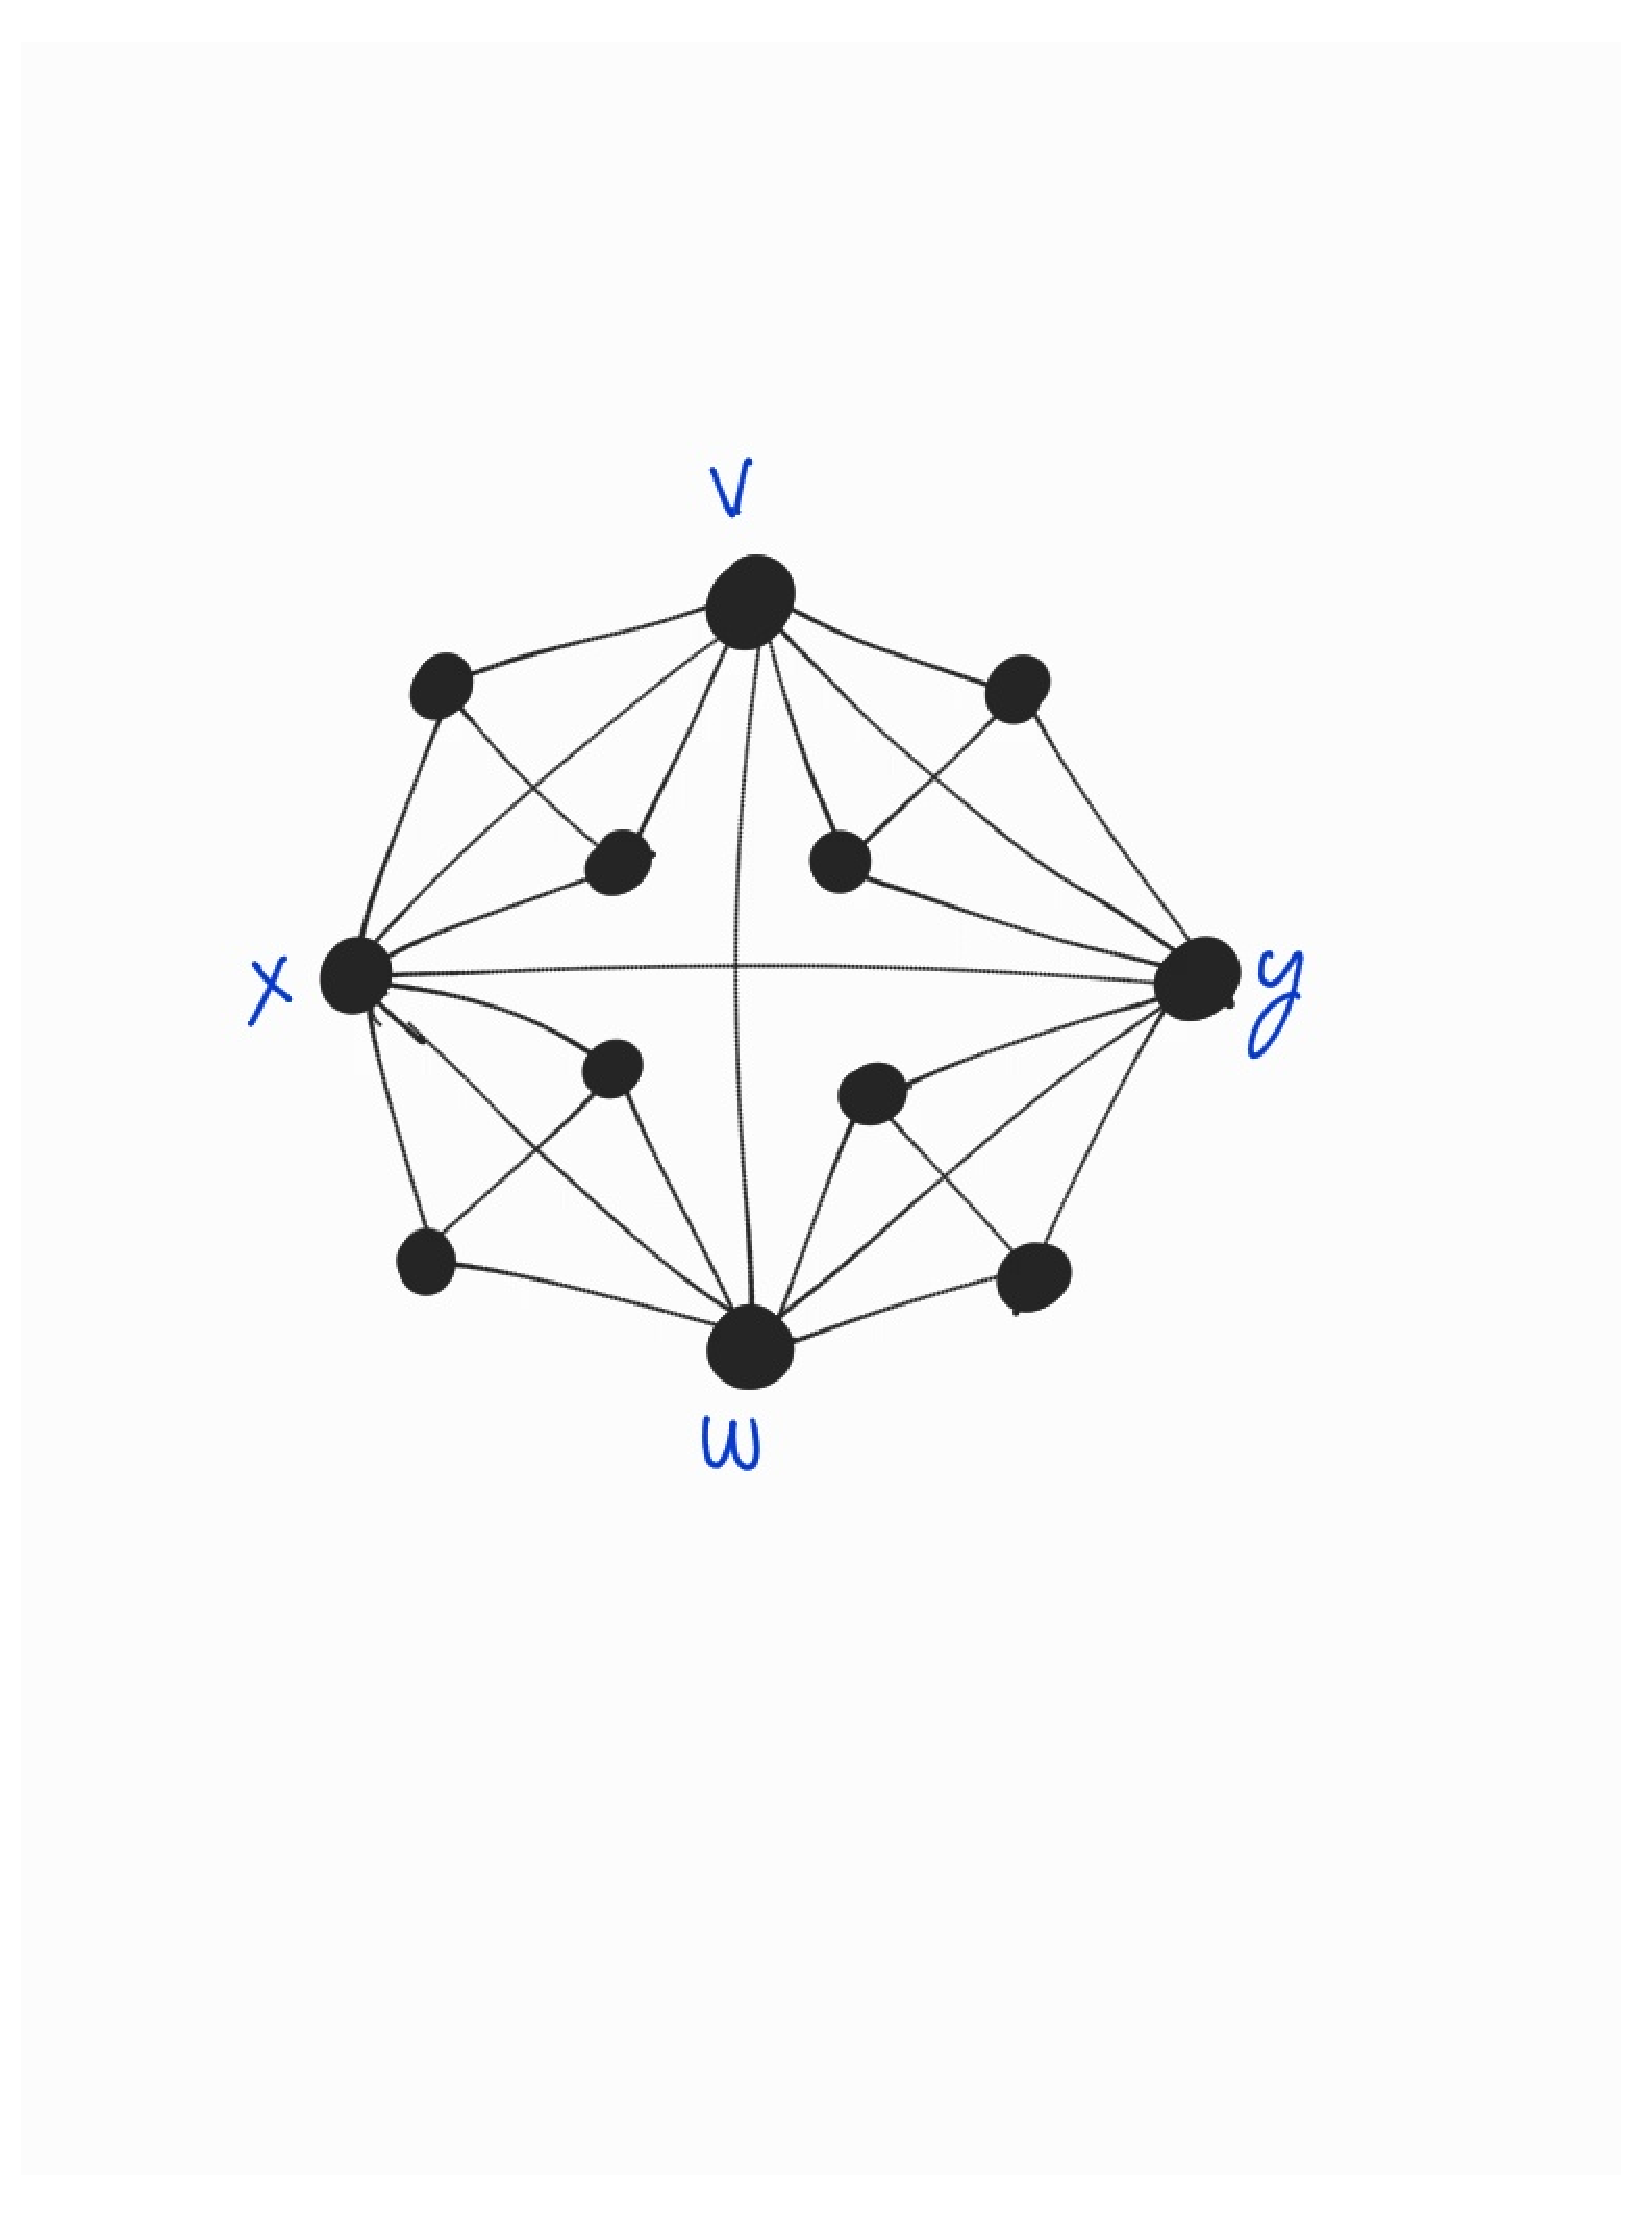
\includegraphics[width=60mm]{kite}}
%\note{DW}{We need to explain more about how edge-maximality fixes this problem. In this case we can draw other $xv$, $vy$, $yw$ $wx$ edges close to the central crossing edges.} Thus any edge that is a spar of a kite $K$ is not part of a sail of any kite $K'$.
%
%\referee{2}{Page 13. The attached PDF also shows that the definition of 'kite
%face' may not be well-defined.  For example, I do not see why there
%cannot be some edges of $G$ 'inside' a kite face.  Even if this is not
%the case, I think it is more precise to say that a kite face has 'two
%and a half edges' and two vertices of $G$ on its boundary' rather than
%'three edges and two vertices of $G$ on its boundary'.}
%
%\note{DW}{This should be fixed if we define kite more precisely. A kite-face is bounded by one edge and two half-edges right?}


Let $G$ be an edge-maximal $1$-plane multigraph with no two parallel edges on the boundary of a single face.  Here, edge-maximal should be taken to mean that, if any two vertices $v$ and $w$ appear on a common face\footnote{The \defin{faces} of an embedded graph $G$ are the connected components of $\R^2\setminus \bigcup_{vw\in E(G)} vw$.  We say that a vertex $v\in V(G)$ appears on a face $F$ if $v$ is contained in the closure of $F$.} $F$, then there is an edge $vw\in E(G)$ that is contained in the boundary of $F$.  (Refer to \cref{one_planar_example}(a,b).) We assume that no two edges incident to a common vertex of $G$ cross each other since, in a 1-plane graph, such a crossing can always be removed by a local modification to obtain an isomorphic 1-plane graph in which the two edges do not cross.\footnote{While this is true for 1-plane graphs it is not true for $k$-plane graphs with $k\ge 3$; the uncrossing operation can increase the number of crossings on a particular edge from $k$ to $2(k-1)$.}

\begin{figure}
  \begin{center}
    \begin{tabular}{c@{\hspace{1cm}}c}
      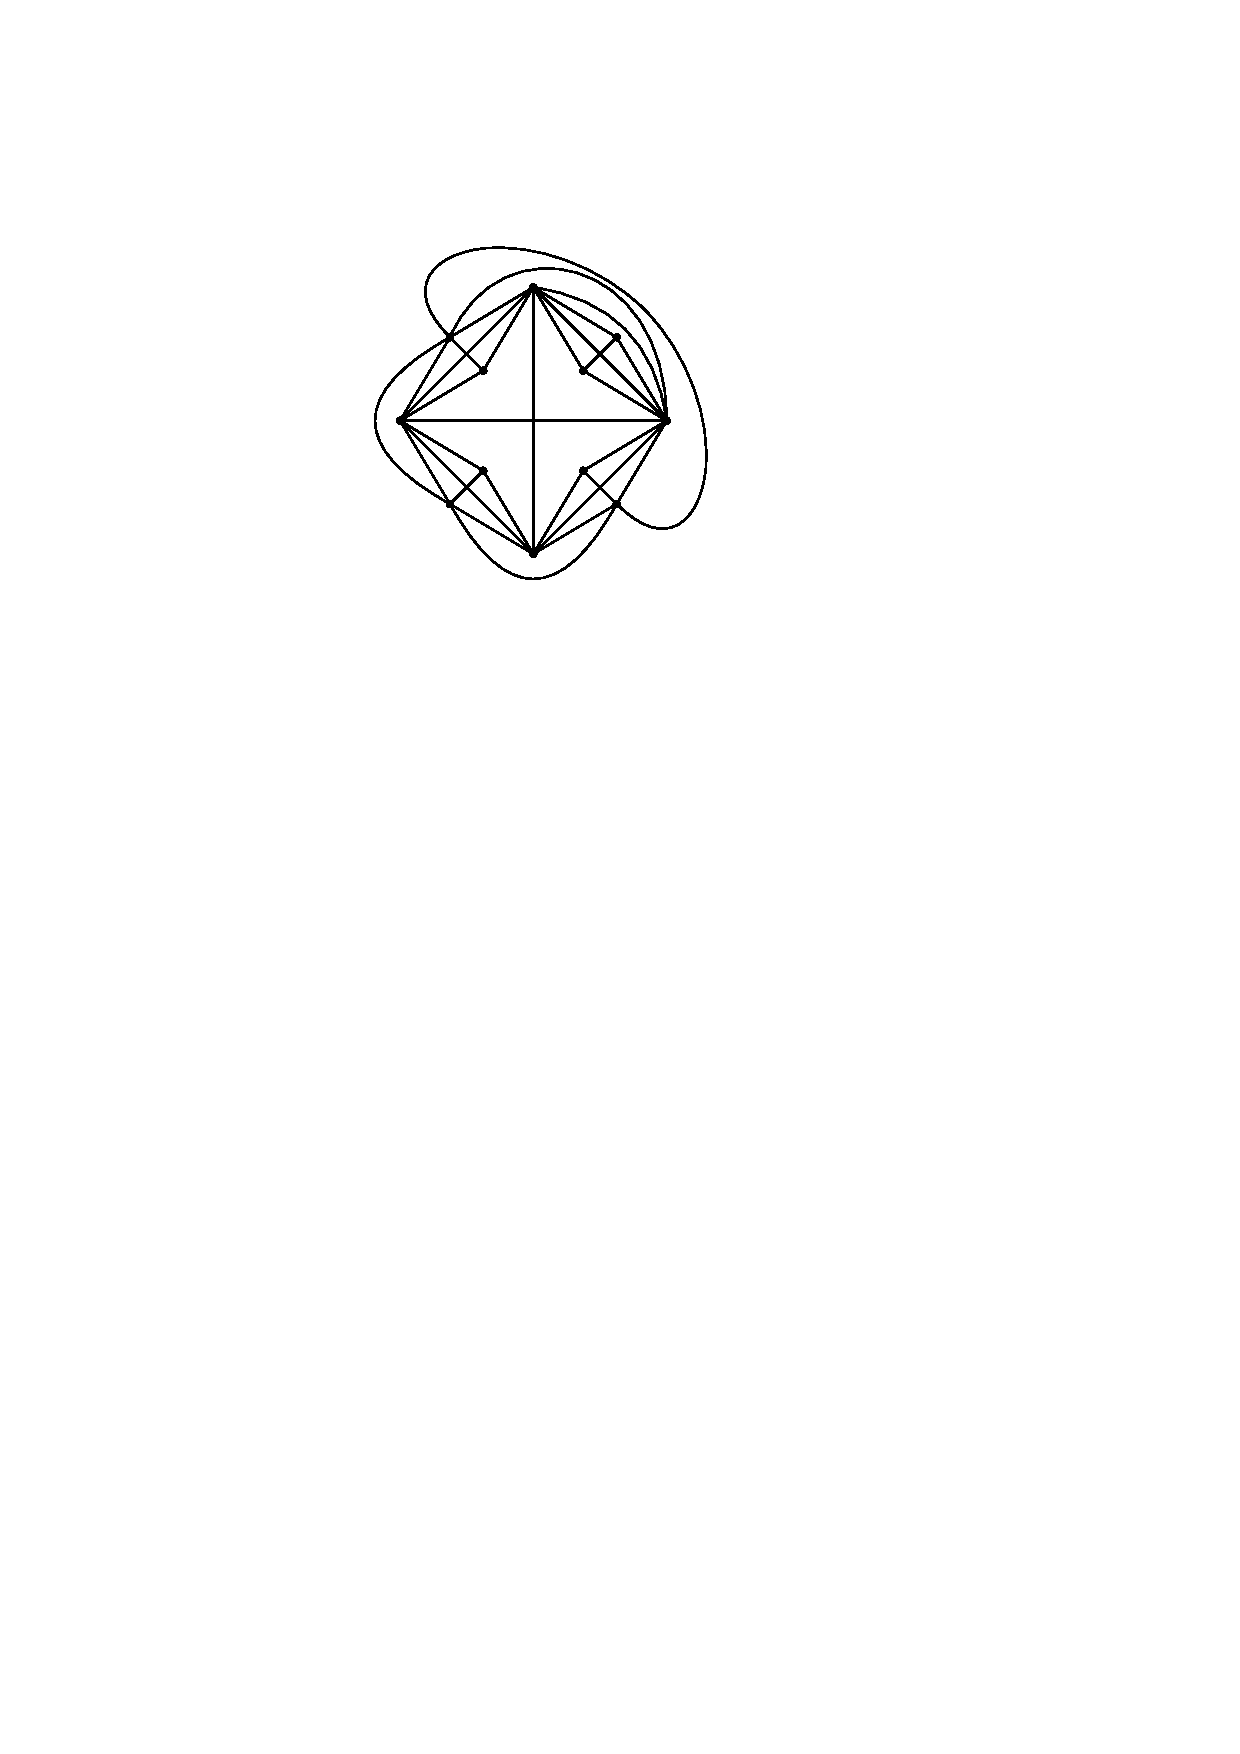
\includegraphics{figs/one_planar_example-1} &
      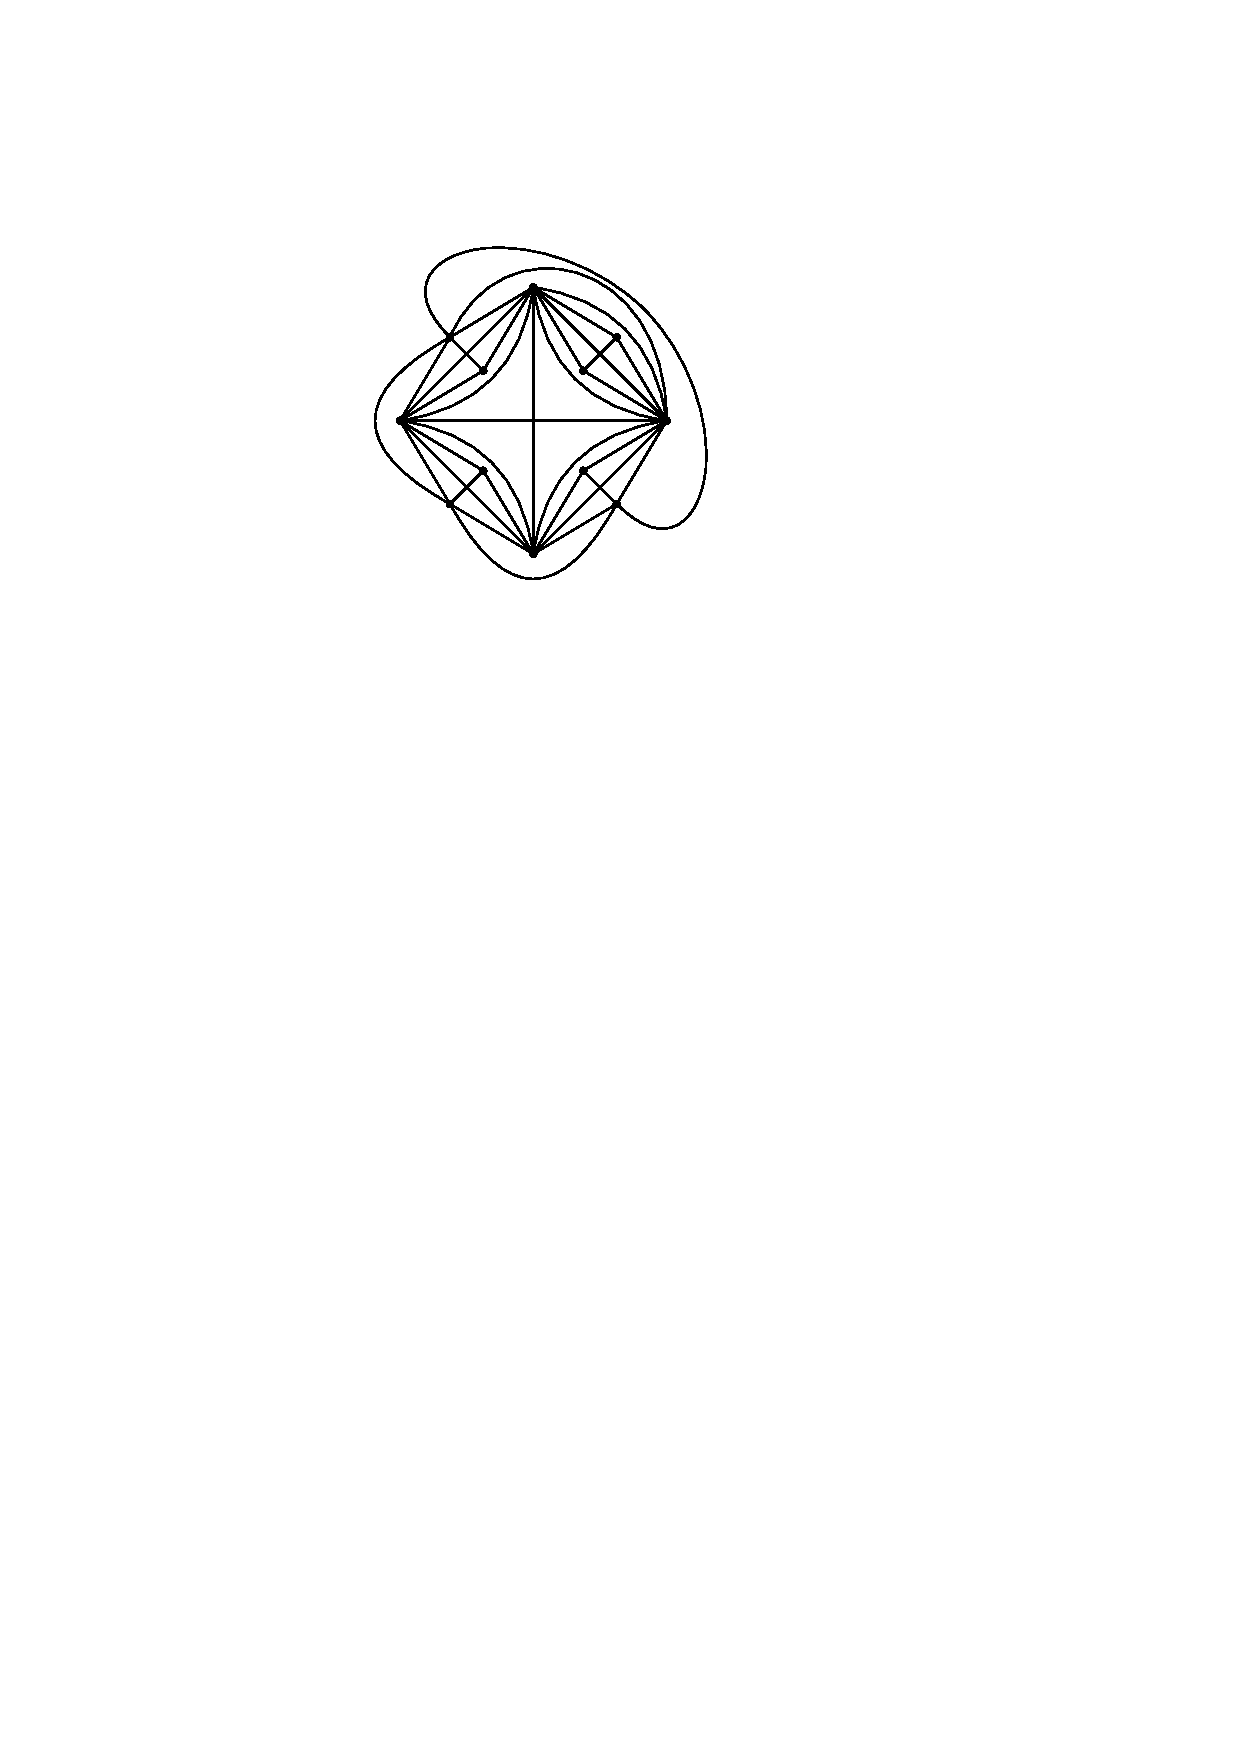
\includegraphics{figs/one_planar_example-2} \\
      (a) & (b) \\[1em]
      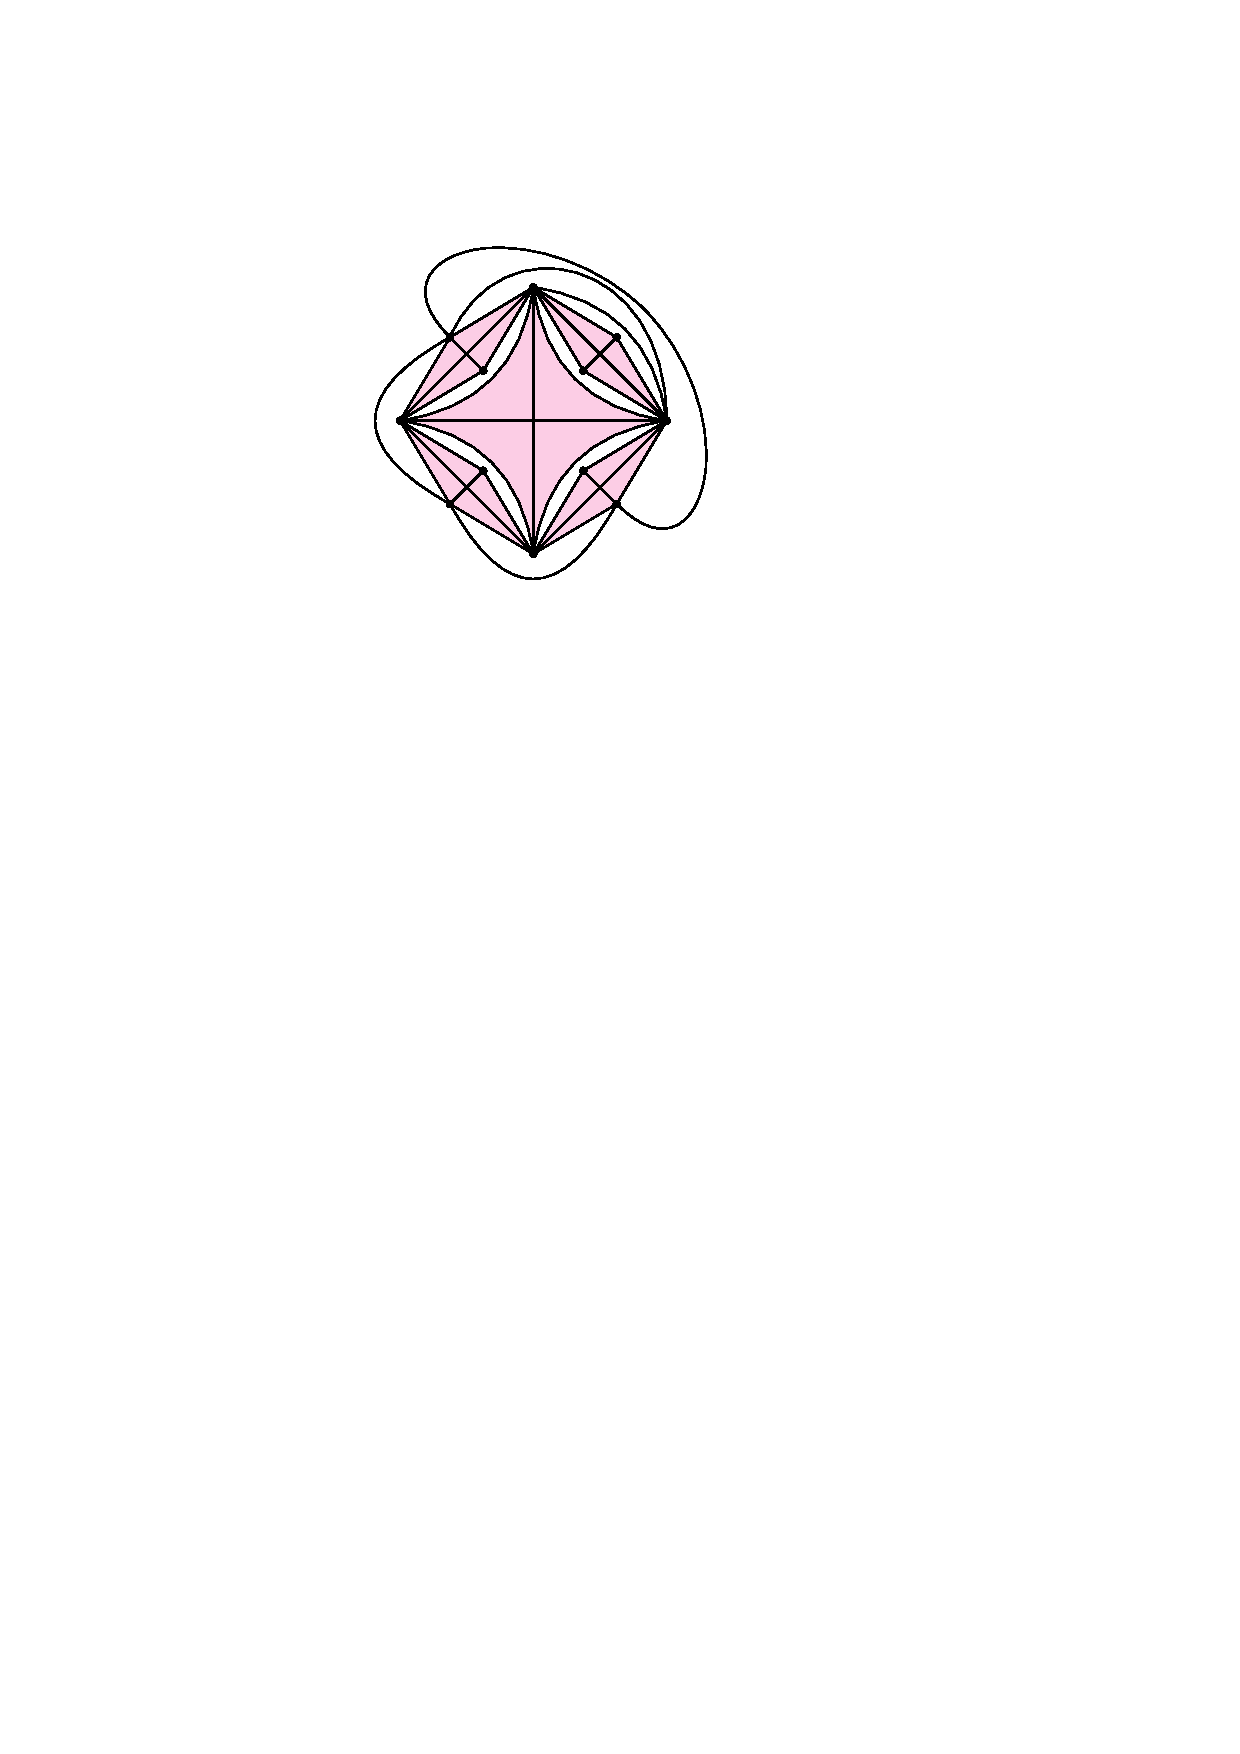
\includegraphics{figs/one_planar_example-3} &
      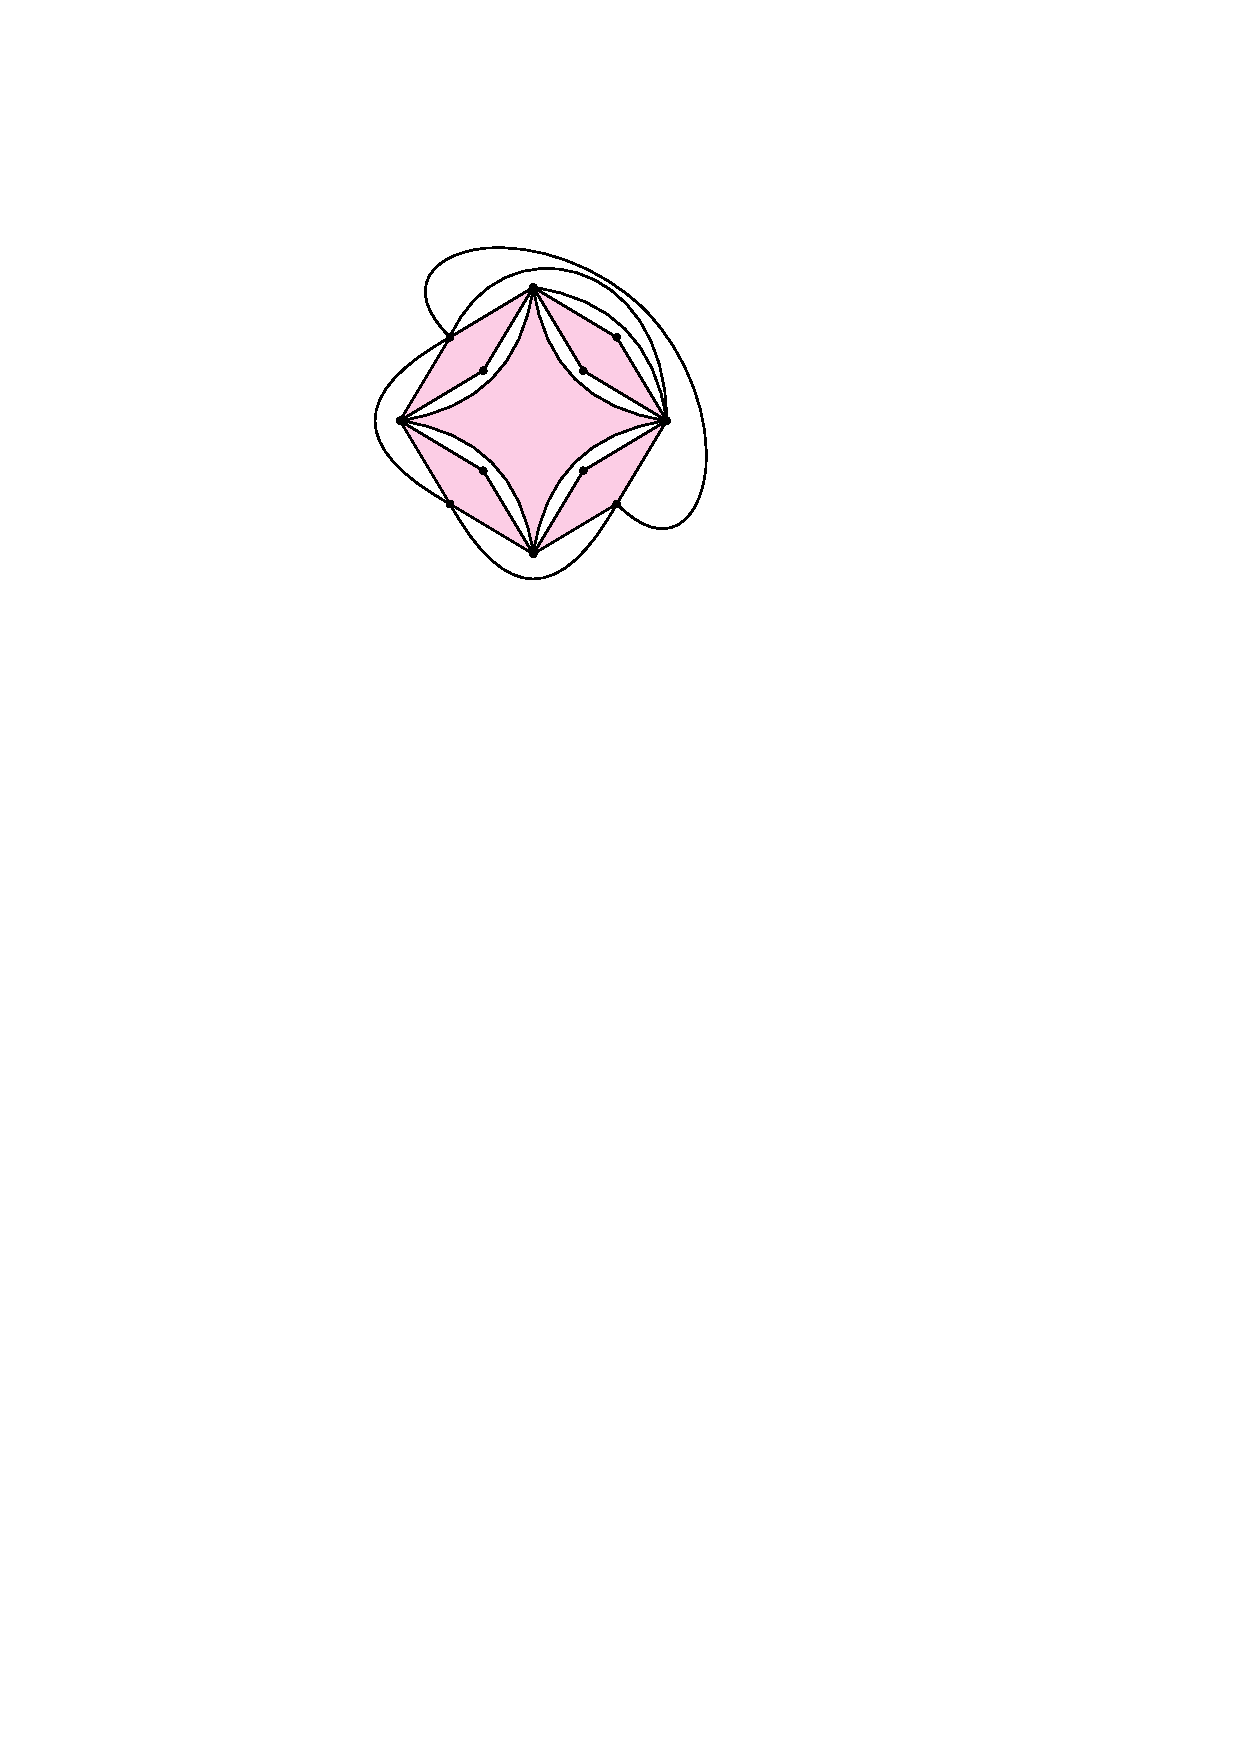
\includegraphics{figs/one_planar_example-4} \\
      (c) & (d) \\[1em]
    \end{tabular}
  \end{center}
  \caption{Examples of (a)~a $1$-plane graph that is not edge maximal; (b)~an edge-maximal $1$-plane graph $G$; (c)~the kites in $G$; (d)~a plane multigraph $G'$ obtained by removing one spar from each kite of $G$.} 
  \label{one_planar_example} 
  \note{PM}{I suggest we only keep parts (c) and (d) of this figure.}
\end{figure}

To understand the structure of $G$, it is helpful to consider the plane graph $G_0$ obtained by replacing each pair of edges $vw$ and $xy$ involved in a crossing $(p,vw,xy)$ with four edges $vp$, $wp$, $xp$, and $yp$ meeting at a newly added \emph{dummy vertex} $p$. Let $F$ be a face of $G_0$ and let $W:=w_0,\ldots,w_r$ be the facial walk around $F$. By edge maximality, if $W$ contains only non-dummy vertices, then it contains exactly three vertices and $F$ is bounded by three edges of $G$. 

If $W$ contains a dummy vertex $w_i$ then neither $w_{i-1}$ nor $w_{i+1}$ is a dummy vertex since if $w_{i-1}$ (respectively $w_{i+1}$) were a dummy vertex then the edge of $G$ that contains $w_{i-1}w_i$ (respectively $w_iw_{i+1}$) is involved in at least two crossings.  Therefore each dummy vertex $w_i$ of $W$ is surrounded by two vertices $w_{i-1},w_{i+1}\in V(G)$.  Since $w_i$ has degree $4$ in $G_0$, $w_{i-1}\neq w_i$.  Since $G$ is edge-maximal the edge $w_{i-1}w_i$ is an edge of $G$ on the boundary of $F$.  Therefore, if $F$ has a dummy vertex $w_i$ in its facial walk $W$, then $W=w_{i-1},w_i,w_{i+1}$ and $F$ is bounded by three edges of $G_0$, each of which is contained in a different edge of $G$.  

Therefore, each face of $G$ is one of two types:
\begin{inparaenum}[(i)] 
  \item bounded by three edges of $G$ (none of which are crossed) or 
  \item bounded by one edge of $G$ that is not crossed plus portions of two edges of $G$ that cross each other.
\end{inparaenum}
Consider some crossing $(p,vw,xy)$ in $G$.  The point $p$ at which this crossing occurs is a vertex of $G_0$ that has degree $4$.  There are four faces $F_1,\ldots,F_4$ of $G_0$ that contain $p$.  Each of these four faces of is of Type~(ii), so the boundary of $F_1\cup\cdots\cup F_4$ includes a $4$-cycle $C:=vxwy$ in $G$ whose edges are not involved in any crossings.  We call the subgraph $K:=C\cup\{vw,xy\}$ a \defin{kite} of $G$. (See \cref{one_planar_example}(c).)  The edges $vw$ and $xy$ are called \defin{spars} of $K$.  The cycle $vxwy$ is called the \defin{sail} of $K$.  Thus any edge that is a spar of a kite $K$ is not part of a sail of any kite $K'$.


\note{PM}{I've commented out a lot of red and blue here to make this readable. Those notes are still in the \LaTeX\ source.}
% 
% It follows from edge-maximality that none of the edges $vx$, $xw$, $wy$, or $yv$ are crossed by any other edges of $G$. 

% 
% \note{DW}{Each face of $G$ is one of two types, either bounded by three edges (none of which are crossed), or bounded by one edge that is not crossed plus portions of two crossing edges. Right? If this is true, we should say it here, which would help to clear up the confusion below. Add a figure.}
% 
% \note{DW}{I suggest we say that it follows from Euler's formula that $G$ is finite. (To see this, say $G$ has $n$ vertices, $m$ non-crossed edges, and $k$ crossings. Let $G'$ be the plane graph obtained from $G$ by adding a dummy vertex at each crossing. So $G'$ is a plane multigraph in which every face is bounded by a 3-cycle. It follows from Euler's formula that $m+4k = |E(G')| = 3( |V(G')|-2) = 3 ( n+k-2)$, implying	$m+k = 3 (n-2)$ and $|E(G)| = m+2k \leq 6(n-2)$, which can also be shown by deleting one edge from each crossing point. ) }
% 
% \note{DW}{It seems to be that $G$ can be obtained from a plane multigraph with faces of size 3 or 4 such that no edge is in two 3-faces, by adding a pair of crossing edges across each 4-face. I think this characterises edge-maximal 1-planar multigraphs with no 2-faces. Right? Does this viewpoint help? Is it known?}
% 
% \note{DW}{Say $G$ is obtained from a plane multigraph by making each face a clique. Is $G\subseteq H \boxtimes P \boxtimes K_{f(\omega(G)}$? for some treewidth 3 graph $H$.}
% 
% % A \defin{kite} in $G$ is the subgraph $K=G[\{v,w,x,y\}]$ induced by the endpoints of a pair of crossing edges $vw,xy\in E(G)$.  It follows from edge-maximality that every kite is isomorphic to the complete graph $K_4$. \note{DW}{We need to define a kite to be the subgraph with vertex-set $\{v,w,x,y\}$ and edge-set $\{vx,xy,vx,vy,wy,wx\}$ where $vx,vy,wy,wx$ are the edges on the `outside' of the kite-faces. Then it really is a simple $K_4$. I think this is what we intended. We should add a figure showing a kite and kite-faces. }
% 
% \referee{2}{Page 13. Perhaps I am misunderstanding something, but I do not see why
% 'none of the edges $vx$, $xw$, $wy$, or $yv$ are crossed by any other edges of
% $G$.'  For example, see the attached PDF for a picture where $vw$, $xw$, $wy$,
% and $yv$ are all crossed by other edges of $G$.\\
% 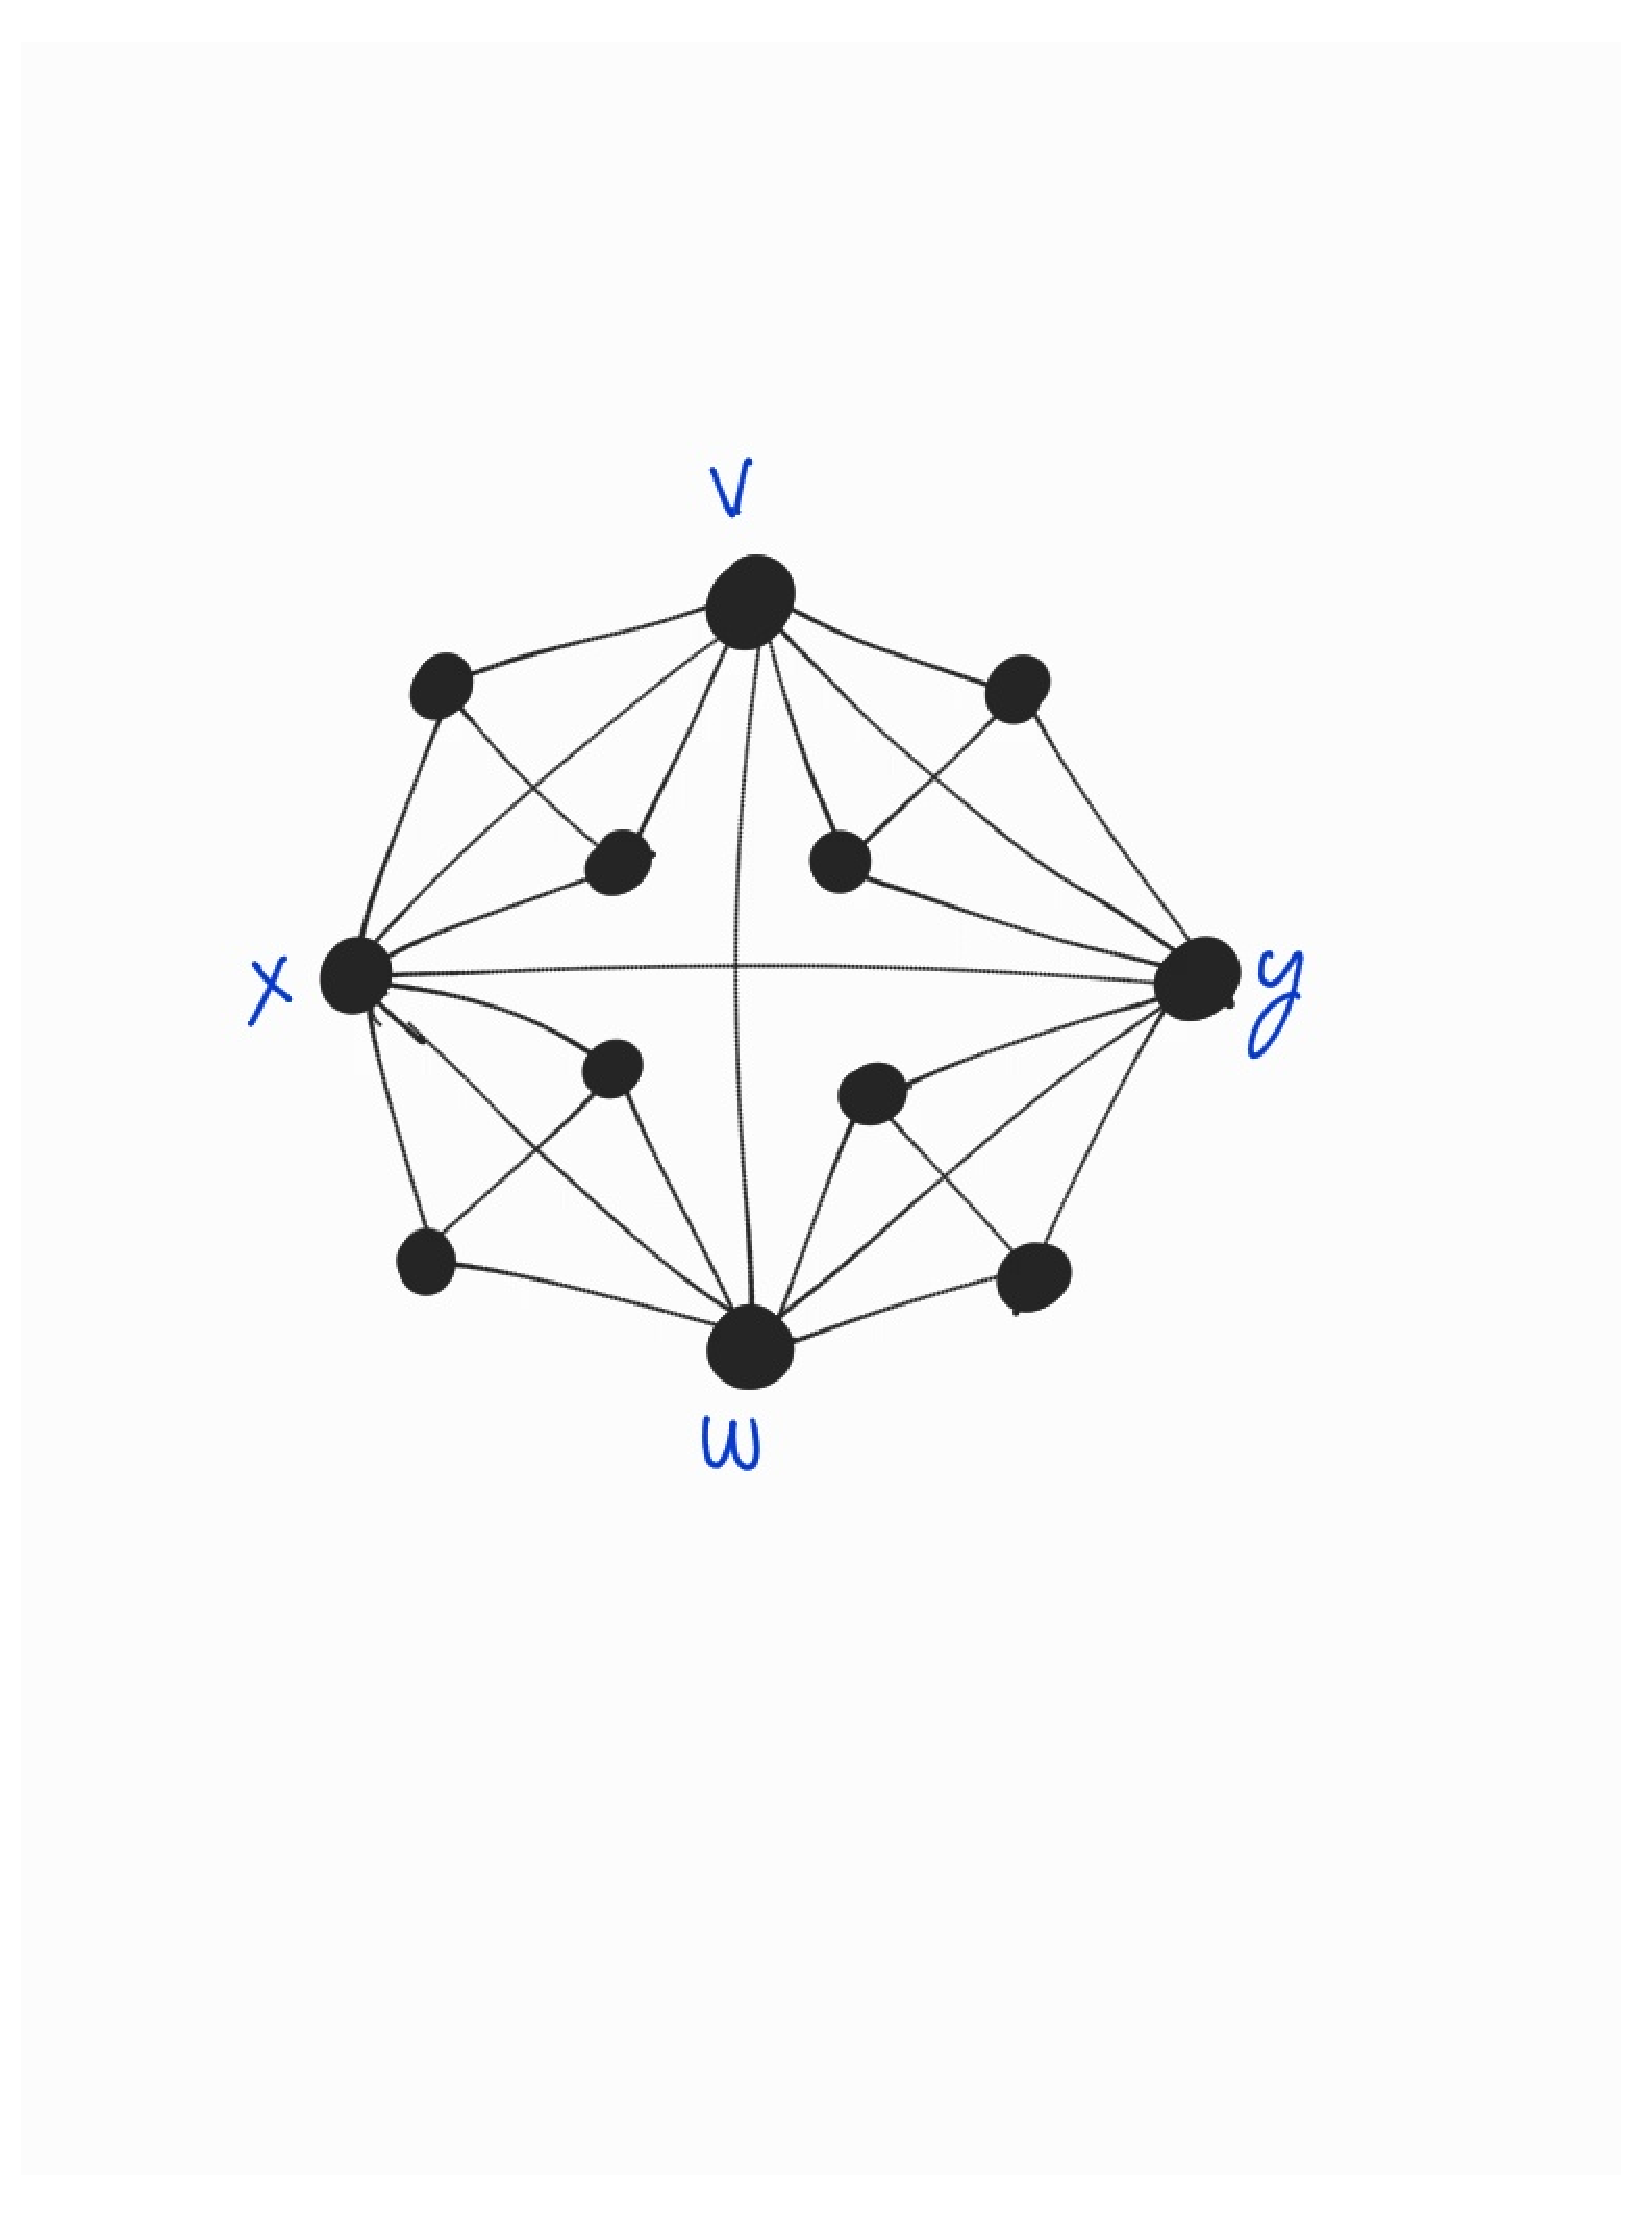
\includegraphics[width=60mm]{kite}}
% \note{DW}{We need to explain more about how edge-maximality fixes this problem. In this case we can draw other $xv$, $vy$, $yw$ $wx$ edges close to the central crossing edges.} \note{PM}{In the example above, $v$ and $y$ appear on a common (inner) face $F$, so by definition of edge-maximality there is an edge $xy$  on the boundary of $F$. }
% 
% \referee{2}{Page 13. The attached PDF also shows that the definition of 'kite
% face' may not be well-defined.  For example, I do not see why there
% cannot be some edges of $G$ 'inside' a kite face.  Even if this is not
% the case, I think it is more precise to say that a kite face has 'two
% and a half edges' and two vertices of $G$ on its boundary' rather than
% 'three edges and two vertices of $G$ on its boundary'.}
% \note{DW}{This should be fixed if we define kite more precisely. A kite-face is bounded by one edge and two half-edges right?}
% 
% \referee{2}{Page 13. Could it be that the subgraph induced by the vertices of a
% 	kite is a $K_4$ with some parallel edges?  This seems relevant later in
% 	the proof.}
% 
% \note{DW}{If we define kite as above, this is not a problem}

Refer to \cref{one_planar_example}(d).  By removing one spar from each kite of $G$ we obtain a plane multigraph $G'$ each of whose faces is bounded by three edges.  Observe that, for any spar $xy\in E(G)\setminus E(G')$ that crosses $vw\in E(G')$, $G'$ contains the path $vxw$ (and $vyw$).  It follows that $\dist_{G'}(v,w)\le 2$.

Our proof of \cref{1-planar} follows quickly from the following technical lemma, which is an extension of the analogous result for plane graphs \cite{DJMMUW20}. 
\begin{lem}
	\label{induction} The setup:
	\begin{compactenum}
		\item Let $G$ and $G'$ be defined as above.
		\item Let $T$ be a BFS spanning tree of $G'$ rooted at some vertex $r$.
		\item For every integer $j\ge 0$, let $L_j=\{v\in V(G):\dist_T(r,v)=j\}$.
		\item Let $F$ be a cycle in $G'$ with $r$ in the exterior of $F$ and such that
		\begin{compactenum}
			\item No edge of $F$ is crossed by any edge of $G$; and
			\item $V(F)$ can be partitioned into $P_1,\ldots,P_k$, for some $k\in\{1,2,3\}$ such that for each $i\in\{1,\ldots,k\}$,
			\begin{compactenum}
				\item $F[P_i]$ is a path; and
				\item $|V(P_i)\cap L_j| \le 15$ for every integer $j\ge 0$.
			\end{compactenum}
		\end{compactenum}
	\note{DW}{Should the vertices already grabbed by $P_1,P_2,P_3$ be mentioned in the setup? The new paths $Q_1,Q_2,Q_3$ need to avoid the vertices already grabbed by $P_1,P_2,P_3$. Basically, I am concerned about what happens when distinct vertical paths in $T$ want to grab the same vertex.}
  \note{PM}{No, at this point we're only promising an $H$-partition of $N$, the part of $G$ contained in the uncrossed cycle $F$.}
		\item Let $N$ and $N'$ be the subgraphs of $G$ and $G'$ consisting only of those edges and vertices contained in $F$ or the interior of $F$.
	\end{compactenum}
	Then $N$ has an $H$-partition $\mathcal{P}=\{S_x : x\in V(H)\}$ such that:
	\begin{compactenum}
		\item $H$ is planar;
		\item for every integer $j\ge 0$ and every $x\in V(H)$, $|S_x\cap L_j|\le 15$;
		\item for each $i\in\{1,\ldots,k\}$, there exists some $x_i\in V(H)$ such that $P_i=S_{x_i}$
		\note{DW}{Should this be $P_i\subseteq S_{x_i}$? (since the path grabs other vertices into its part)}\note{PM}{No, for the same reason as above.}; and
		\item $H$ has a tree-decomposition in which every bag has size at most 4 and such that some bag contains $x_1,\ldots,x_k$.
	\end{compactenum}
\end{lem}

\referee{2}{Page 13.  Regarding the proof of Lemma 4, I think it is better to
include all the details from reference [14].  As far as I know, JCTB
does not have a page limit, so I do not see an issue with just
reproducing the entire proof and telling the reader that they can skip
all the details if they wish.  This is just my personal opinion
though, so the authors can ignore this request if they choose.}

\note{DW}{I agree we need more details. I am having trouble verifying this proof. }

\begin{proof}
	This proof is very similar to the proof of Lemma~14 by \citet{DJMMUW20}, but is sufficiently complicated by the $1$-planar setting to warrant a full proof.
   % 
   % 
   % 
   % 
   % Rather than duplicate every detail of that proof here, we focus on the differences and refer the reader to the original proof for the remaining details.
  In particular, the reader should keep in mind that $G$ and $G'$ are multigraphs and that the cycle $F$ may consist of two vertices and two (parallel) edges. 	
  
  The proof is by induction on the number of inner vertices of $N$, i.e., on $|V(N)\setminus V(F)|$.  If $N$ has no inner vertices, then we can simply take $\mathcal{P}:=\{P_1,\ldots,P_k\}$ and verify the preconditions of the lemma (the setup) ensure that $\mathcal{P}$ satisfies the requirements of the lemma.  Therefore, we may assume that $N$ has at least one inner vertex.
  
	First note that every inner face of $N'$ is bounded by three edges of $G'$. 
  Assign each vertex $v$ of $N'$ a colour $\alpha(v)\in\{1,2,3\}$ as follows: 
  Let $w$ be the first vertex of $F$ encountered on the path in $T$ from $v$ to the root of $T$.  (This implies that $w=v$ for $v\in V(F)$.)  Since $w\in V(F)$, $w\in P_i$ for some $i\in\{1,2,3\}$ and we define $\alpha(v):=i$.
  
  If $k<3$ then let $\tau:=v_1v_2v_3$ be any inner face of $N'$.  Otherwise, $k=3$, in which case we apply Sperner's Lemma implies to obtain an inner face $\tau:=v_1v_2v_3$ such that $\alpha(v_i)=i$ for each $i\in\{1,2,3\}$.  
  For each $i\in\{1,2,3\}$, let $Q_i$ be the shortest path, in $T$, from $v_i$ to $V(F)$.
   % 
   % 
   % If $k=3$, set $R_i := P_i$ for each $i\in\{1,2,3\}$.  Otherwise, as in \citep{DJMMUW20}, split $P_1,\ldots,P_k$ to partition $V(F)$ into three sets $R_1$, $R_2$, and $R_3$ such that each $F[R_i]$ is a non-empty path and each $R_i$ contains vertices from exactly one of $P_1,\ldots,P_k$.
  % 
	% Next, as in \citep{DJMMUW20}, use Sperner's Lemma to find an inner face $\tau=v_1v_2v_3$ of $N'$ such that, $T$ contains disjoint vertical paths $Q_1,Q_2,Q_3$ such that each $Q_i$ begins at $v_i$, ends at some vertex in $R_i$, and whose internal vertices (if any) are contained in $N'-V(F)$.
	Let $\overline{Y}$ denote the subgraph of $N'$ consisting of vertices and edges of $Q_1$, $Q_2$, $Q_3$, and $\tau$.  Let $\overline{Y}^+$ denote the subgraph of $N$ consisting of the vertices and edges of $\overline{Y}$ plus the vertices and edges of every kite formed by a crossing between an edge of $G$ and an edge of $\overline{Y}$.

	We claim that, for each integer $i\ge 0$, $|V(\overline{Y}^+)\cap L_i|\le 15$.  First observe that, since $Q_1,Q_2,Q_3$ are each vertical paths in $T$,  $\overline{Y}$ contains at most three vertices of $L_i$, each incident on at most two edges of $\overline{Y}$.  Since $\dist_{G'}(v,w)\le 2$ for each $vw\in E(G)$, any vertex $x\in V(\overline{Y}^+)\setminus V(\overline{Y})\cap L_i$, is incident to an edge $xy\in E(G)$ that crosses one of the at most six edges in $\overline{Y}$ having an endpoint in $L_i$.  These at most six edges have at most 12 endpoints.  Therefore $|V(\overline{Y}^+)\setminus V(\overline{Y})\cap L_i|\le 6\times 2=12$, so $|V(\overline{Y}^+)\cap L_i|\le 12+3=15$.

	Let $M$ and $M^+$ denote the subgraph of $G$ containing the edges and vertices of $\overline{Y}$, respectively $\overline{Y}^+$, and the edges and vertices of $F$.  The graph $M^+$ has some number of bounded faces, all contained in the interior of $F$. Some of the bounded faces of $M^+$ are kite faces. Let $F_1,\ldots,F_m$ be the non-kite bounded faces of $M^+$.

	We claim that, for each $i\in\{1,\ldots,m\}$, the boundary of $F_i$ is a cycle in $G'$ that contains no spars. Otherwise, some edge $vw$ contributes to the boundary of $F_i$ but is crossed by an edge $xy\in E(G)$. Then, $vw\not\in E(F)$ since no edge of $F$ is crossed by any edge of $G$. Therefore $vw\in E(\overline{Y}^+)$ so $xy\in E(Y^+)$. But then the only faces of $M^+$ incident to $vw$ are kite faces.  In particular $vw$ cannot be incident to the non-kite face $F_i$.

	Observe that each of the faces $F_1,\ldots,F_m$ is contained in a single internal face of $M$.   Let $Y^+ := \overline{Y}^+-F$. Therefore, $V(F_i)$ can be partitioned into at most three sets $P_1'$, $P_2'$, and $P_3'$ where $P_1'\subset V(Y^+)$, $P_2'\subseteq P_a$, $P_3'\subseteq P_b$ for some $a,b\in\{1,2,3\}$, and $F_i[P_j']$ is a path, for each $j\in\{1,2,3\}$.

	Finally, the subgraph $N_i$ of $G$ consisting of the edges and vertices of $G$ contained in $F_i$ or its interior does not contain one of the three vertices of $\tau$. Therefore, we can apply induction using the cycle $F_i$ and the partition $P_1',P_2',P_3'$ of $V(C_i)$ to obtain the desired $H$-partition and tree decomposition of $N_i$.

	The proof finishes in the same way as the proof in \cite{DJMMUW20}.  The paths $P_1,\ldots,P_k$, and $S=V(Y^+)$ become elements of the $H$-partition.
	Elements in each of the $H$-partitions of $N_1,\ldots,N_3$ that intersect $P_1,\ldots,P_k$, or $V(\overline{Y}^+-F)$ are discarded and all the resulting sets are combined to obtain an $H$-partition of $G$.  The desired tree decomposition of $G$ is obtained in exactly the same way as in the proof of Lemma~14 in \cite{DJMMUW20}, except that now each node $x$ has a child for each face $F_i$ of $M^+_x$ that contains a vertex of $G$ in its interior.

	\note{DW}{Check whether Lemma~14 is the right lemma}

	The planarity of $H$ comes from two properties:
	\begin{compactenum}
		\item $G/\mathcal{P}$ and $G^+/\mathcal{P^+}$ are isomorphic, where $G^+$ is the triangulation obtained by adding dummy vertices at each crossing in $G$ and $\mathcal{P}^+$ is the partition we obtain by adding a dummy vertex $z$ to $\overline{Y}^+$ if $\overline{Y}^+$ contains an edge $vw$ that contains $z$ in its interior.

		\item $G^+[\overline{Y}^+-F]$ is connected. To see this, first observe that $\overline{Y}-F$ is connected, and then observe that every vertex of $\overline{Y}^+$ is either a vertex of $\overline{Y}$ or adjacent to a vertex of $\overline{Y}$.
	\end{compactenum}
	Since $G^+$ is planar, the second point implies that $H=G^+/\mathcal{P}$ is planar.
	% \footnote{It is well-known and easy to see that any graph $\Delta'$ obtained by contracting an edge in a planar graph $\Delta$ is also planar.  Repeatedly applying this fact implies that $\Delta/\mathcal{P}$ is planar provided that $\Delta[P]$ is connected for every $P\in\mathcal{P}$.} The first point then ensures that $G/\mathcal{P}$ is also planar.
	\note{DW}{We need a sentence about why $H$ Has the claimed tree-decomposition.}
\end{proof}

Using \cref{induction}, the proof of \cref{1-planar} is now straightforward.

\begin{proof}[Proof of \cref{1-planar}]
	Given a 1-plane graph $G$, add edges to make it edge-maximal so that it has an outer face $F=v_1v_2v_3$. Next, add a vertex $r$ adjacent to $v_1$, $v_2$, and $v_3$ to obtain an edge-maximal 1-plane graph $\overline{G}$ with one vertex $r$ of degree 3 on its outer face.

	Let $G'$ be the plane graph obtained by removing one spar from each kite of $\overline{G}$ and let $T$ be a BFS tree of $G'$ rooted at $r$.  Now apply \cref{induction} with $G=\overline{G}$, $G'$, $F$, and $P_i=\{v_i\}$ for each $i\in\{1,2,3\}$.  This gives an $H$-partition $\{S_x:x\in V(H)\}$ of $\overline{G}-\{r\}\supseteq G$ in which $H$ is planar and has treewidth at most 3.

	Use the layering $\mathcal{L}=\langle L_0',L_1'\ldots\rangle$ where $L_i'=L_{2i}\cup L_{2i+1}$ for each integer $i\ge 0$. That this is a layering of $G$ follows from the fact that $\dist_{G'}(v,w)\le 2$ for every edge $vw\in E(G)$.  Since $|L_j\cap S_x|\le 15$ for every integer $j\ge 0$, $|L_i'\cap S_x|\le 30$ for every integer $i\ge 0$ and every $x\in V(H)$. The result follows from \cref{PartitionProduct}.
\end{proof}

\subsection{\boldmath $(g,k)$-Planar Graphs}

The definition of $k$-planar graphs naturally generalises for other surfaces. A graph $G$ drawn on a surface $\Sigma$ is $(\Sigma,k)$-plane if every edge of $G$ is involved in at most $k$ crossings.  A graph $G$ is $(g,k)$-planar if it is isomorphic to some $(\Sigma,k)$-plane graph, for some surface $\Sigma$ with Euler genus at most $g$. \cref{AddDummy} immediately generalises as follows:

\begin{obs}
\label{gAddDummy}
Every $(g,k)$-planar graph $G$ is a subgraph of $G_0^\SS$ for some graph $G_0$ of Euler genus at most $g$ and some $(k+1,2)$-shortcut system $\SS$ for $G_0$. Moreover, $V(G) \subseteq V(G_0)$ and for every edge $vw \in E(G)$ there is a $vw$-path $P$ in $G_0$ of length at most $k+1$, such that every internal vertex in $P$ has degree at most $4$ in $G_0$.
\end{obs}

Theorems~\ref{ShortcutProduct}  and \ref{GenusProduct}(b) imply a product structure theorem for $(g,k)$-planar graphs. The obtained bounds are improved by the following result, which is proved using exactly the same approach used in the proof of \cref{kPlanarProduct} (applying \cref{GenusProduct}(b) instead of \cref{PlanarProduct}(b)). We omit repeating the details.

\begin{thm}
\label{gkPlanarProduct}
Every $(g,k)$-planar graph is a subgraph of $H\boxtimes P \boxtimes K_\ell$ for some graph $H$ with $\tw(H) \leq \binom{k+5}{4}-1$, where $\ell:=\max\{2g,3\}\cdot(6k^2+16k+10)$.
\end{thm}

Prior to this work, the strongest structural description of $k$-planar or $(g,k)$-planar graphs (or any of the other classes presented in \cref{Examples}) was in terms of layered treewidth, which we now define.  A \defin{layered tree-decomposition} $(\mathcal{L},\mathcal{T})$ consists of a layering $\mathcal{L}$ and a tree-decomposition $\mathcal{T}$ of $G$. The layered width of $(\mathcal{L},\mathcal{T})$ is $\max\{|L\cap B|: L\in \mathcal{L},\, B\in \mathcal{T}\}$.  The \defin{layered treewidth} of $G$ is the minimum layered width of any layered tree-decomposition of $G$. \citet{dujmovic.morin.ea:layered} proved that planar graphs have layered treewidth at most 3, that graphs of Euler genus $g$ have layered treewidth at most $2g+3$, and more generally that a minor-closed class has bounded layered treewidth if and only if it excludes some apex graph. \citet{dujmovic.eppstein.ea:structure} show that every $k$-planar graph has layered treewidth at most $6(k+1)$, and more generally that every $(g,k)$-planar graph has layered treewidth at most $(4g+6)(k+1)$. It follows from this result that $(g,k)$-planar graphs have treewidth $O(\sqrt{(g+1)(k+1)n})$ and thus have balanced separators of the same order, which can also be concluded from the work of \citet{FP08}. In related work, \citet{grigoriev.bodlaender:algorithms} used structural results to obtain approximation algorithms for $(g,k)$-planar graphs, and \citet{PachToth97} determined the maximum number of edges in a $k$-planar graph (up to a constant factor).

If a graph class admits bounded layered partitions, then it also has bounded layered treewidth. In particular, if $\mathcal{P}=(P_x:x\in V(H))$ is an $H$-partition of $G$ of layered width $\ell$ with respect to some layering $\mathcal{L}$ of $G$ and $(B_x:x\in V(T))$ is a width-$t$ tree-decomposition of $H$, then setting $C_x = \bigcup_{y\in B_x} P_y$ for each $x\in V(T)$ gives a tree-decomposition $(C_x:x\in V(T))$ of $G$ that has layered treewidth $(t+1)\ell$ \cite{DJMMUW20}. Therefore, any property that holds for graphs of bounded layered treewidth also holds for $G$. What sets layered partitions apart from layered treewidth is that they lead to constant upper bounds on the queue-number  and non-repetitive chromatic number, whereas for both these parameters, the best known upper bound obtainable via layered treewidth is $O(\log n)$; see \cref{Applications}.


\subsection{Rough Characterisation}
\label{Characterisation}

\cref{gAddDummy} shows that $(g,k)$-planar graphs can be obtained by a shortcut system applied to a graph of Euler genus $g$, where internal vertices on the paths have bounded degree. This observation and the following converse result together provide a rough characterisation of $(g,k)$-planar graphs, which is interesting in its own right, and is useful for showing that various classes of graphs are $(g,k)$-planar.

\begin{lem}
	\label{DrawG}
	Fix integers $g\geq 0$ and $k,\Delta\geq 2$.
	Let $G_0$ be a graph of Euler genus at most $g$. Let $G$ be
	a graph with $V(G) \subseteq V(G_0)$ such that for every edge $vw \in
	E(G)$ there is a $vw$-path $P_{vw}$ in $G_0$ of length at most $k$, such
	that every internal vertex on $P_{vw}$ has degree at most $\Delta$ in
	$G_0$. Then $G$ is $(g, 2k(k+1)\Delta^{k} )$-planar.
\end{lem}

\begin{proof}
	For a vertex $x$ of $G_0$ with degree at most $\Delta$, and for $i\in\{1,\dots,k-1\}$, say a vertex $v$ is \defin{$i$-close} to $x$ if there is a $vx$-path $P$ in $G_0$ of length at most $i$ such that every internal vertex in $P$  has degree at most $\Delta$ in $G_0$.
	For each edge $vw$ of $G$, say that $vw$ \defin{passes through} each internal vertex on $P_{vw}$.	Say $vw$ passes through $x$. Then $v$ is $i$-close to $x$ and $w$ is $j$-close to $x$ for some $i,j\in\{1,\dots,k-1\}$ with $i+j\leq k$. At most $\Delta^{i}$ vertices are $i$-close to $x$.
	Thus, the number of edges of $G$ that pass through $x$ is at most
	\[
	\sum_{i=1}^{k-1} \sum_{j=1}^{k-i} \Delta^i \Delta^j
	= \sum_{i=1}^{k-1} \Delta^i  \sum_{j=1}^{k-i} \Delta^j
	< \sum_{i=1}^{k-1} \Delta^i  2 \Delta^{k-i}
	= \sum_{i=1}^{k-1} 2\Delta^k
	< 2k \Delta^k \enspace.
	\]
	Draw each edge $vw$ of $G$ alongside $P_{vw}$ in $G_0$, so that every pair of edges cross at most once.
	Every edge of $G$ that crosses $vw$ passes through a vertex on $P_{vw}$ (including $v$ and/or $w$ if they too have degree at most $\Delta$). Since $P_{vw}$ has at most $k+1$ vertices, and less than $2k\Delta^{k}$ edges of $G$ pass through each vertex on $P_{vw}$, the edge $vw$ is crossed by less than $2k(k+1)\Delta^{k}$ edges in $G$. Hence $G$ is $(g, 2k(k+1)\Delta^{k} )$-planar.
\end{proof}

\referee{2}{Page 16.  At the end of Page 16, I do not see why 'every pair of edges
cross at most once.'  Without further assumptions, it seems as if two
paths in the path system could intersect several times.  Therefore, by
drawing 'each edge vw of G alongside $P_vw$ in $G_0$', there may be two
edges which cross several times.  It seems this can be fixed by
choosing the path system carefully by 'uncrossing' paths which
intersect at more than two internal vertices.}

\note{DW}{But we do not want to uncross. Our claim that ``every pair of edges cross at most once'' is not true. I am convinced the result is still correct. Just need to think  of a better way to write it. Each crossing is in the vicinity of a vertex that has degree $\leq\Delta$. }

%%%%%%%%%%%%%%%%%%%%%%%%
\section{Applications}
\label{Applications}

Here we discuss some of the consequences of the above theorems for $k$-planar and $(g,k)$-planar graphs.

\referee{1}{4. Sections 4 and 5: I think as they are currently organized they distract from the purpose of the paper, as stated in the introduction, to ``prove product structure theorems for several non-minor-closed classes of interest.'' Which of Corollaries 1--4 and Theorems 12--17 are most important? I would remove any mention of the applications from the examples section, put that section first, and state in that section a single main theorem with all of the best bounds on the product structure. The applications section is mostly a survey and I think should be focused on the most exciting new corollaries. Theorems 18 and 19 should be in the applications section.}

\note{DW}{I don't want to do a complete restructuring. In our response, let's just say why we structure it the way we do.}


%%%%%%%%%%%%%%%%%%%
\subsection{Queue Layouts}

For an integer $k\geq 0$, a \textit{$k$-queue layout} of a graph $G$ consists of a linear ordering $\preceq$ of $V(G)$ and a partition $\{E_1,E_2,\dots,E_k\}$ of $E(G)$, such that for $i\in\{1,2,\dots,k\}$, no two edges in $E_i$ are nested with respect to $\preceq$. That is, it is not the case that $v\prec x \prec y \prec w$ for edges $vw,xy\in E_i$. The \textit{queue-number} of a graph $G$, denoted by $\qn(G)$, is the minimum integer $k$ such that $G$ has a $k$-queue layout. Queue-number was introduced by \citet{HLR92}, who famously conjectured that planar graphs have bounded queue-number. \citet{DJMMUW20} recently proved this conjecture using \cref{PlanarProduct} and the following lemma. Indeed, resolving this question was the motivation for the development of \cref{PlanarProduct}.

\begin{lem}[\citep{DJMMUW20}]
\label{qn}
If $G\subseteq H \boxtimes P \boxtimes K_\ell$ then
$\qn(G) \leq  3 \ell \, \qn(H) + \floor{\tfrac{3}{2}\ell}
\leq 3 \ell \, 2^{\tw(H)}  - \ceil{\tfrac{3}{2}\ell}$.
\end{lem}

\cref{qn,gkPlanarProduct} imply that $(g,k)$-planar graphs have queue-number at most $g 2^{O(k^4)}$.

Note that \citet{DJMMUW20} previously proved the bound of
$O(g^{k+2})$ using \cref{GenusProduct} and an ad-hoc method. Our result provides a better bound when $g>2^{k^3}$. In the case of 1-planar graphs we can improve further. \citet{ABGKP20} proved that every planar graph with treewidth at most $3$ has queue-number at most $5$. Thus the graph $H$ in \cref{1-planar} has queue-number at most $5$. \cref{qn,1-planar} then imply:

\begin{cor}
\label{1PlanarQueue}
Every 1-planar graph has queue-number at most $3 \times 30 \times 5 + \floor{\tfrac{3}{2} \times 30} = 495$.
\end{cor}


%%%%%%%%%%%%%%%%%%%
\subsection{Non-Repetitive Colouring}

The next two applications are in the field of graph colouring. For our purposes, a \defin{$c$-colouring} of a graph $G$ is any function $\phi\colon V(G)\to C$, where $C$ is a set of size at most $c$.
A $c$-colouring $\phi$ of $G$ is \defin{non-repetitive} if, for every path $v_1,\ldots,v_{2h}$ in $G$, there exists $i\in\{1,\ldots,h\}$ such that $\phi(v_i)\neq\phi(v_{i+h})$.  The \defin{non-repetitive chromatic number} $\pi(G)$ of $G$ is the minimum integer $c$ such that $G$ has a non-repetitive $c$-colouring. This concept, introduced by \citet{AGHR-RSA02}, has since been widely studied; see \citep{dujmovic.esperet.ea:planar} for more than 40 references. Up until recently the main open problem in the field has been whether planar graphs have bounded non-repetitive chromatic number, first asked by \citet{AGHR-RSA02}. \citet{dujmovic.esperet.ea:planar} recently solved this question using \cref{PlanarProduct} and the following lemma.

\begin{lem}[\citep{dujmovic.esperet.ea:planar}]
\label{non-repetitive}
If $G\subseteq H\boxtimes P \boxtimes K_\ell$ then $\pi(G)\le \ell\, 4^{\tw(H)+1}$.
\end{lem}

\cref{non-repetitive,kPlanarProduct,1-planar,gkPlanarProduct} imply the following result:

\begin{cor}\quad
\begin{compactitem}
\item	For every $1$-planar graph $G$, $\pi(G)\le 30\times 4^4=7680$.
\item For every $k$-planar graph $G$,
	$\pi(G)\le (18k^2+48k+30) 4^{\binom{k+4}{3}}$.
\item	For every $(g,k)$-planar graph $G$,
	$  \pi(G)\le \max\{2g,3\}\cdot(6k^2+16k+10) 4^{\binom{k+5}{4}}.$
\end{compactitem}
\end{cor}

Prior to the current work, the strongest upper bound on the non-repetitive chromatic number of $n$-vertex  $k$-planar graphs was $O(k\log n)$ \cite{dujmovic.morin.ea:layered}.

%%%%%%%%%%%%%%%%%%%
\subsection{Centered Colourings}
\seclabel{centered-colourings}

A $c$-colouring $\phi$ of $G$ is \defin{$p$-centered} if, for every connected subgraph $X\subseteq G$, $|\{\phi(v):v\in V(X)\}| > p$ or there exists some $v\in V(X)$ such that $\phi(v)\neq \phi(w)$ for every $w\in V(X)\setminus\{v\}$.  In words, either $X$ receives more than $p$ colours or some vertex in $X$ receives a unique colour.  Let $\chi_p(G)$ be the minimum integer $c$ such that $G$ has a $p$-centered $c$-colouring. Centered colourings are important since they characterise classes of bounded expansion, which is a key concept in the sparsity theory of \citet{Sparsity}.

\citet{PS21} and \citet{DFMS21} use \cref{ps} and \cref{PlanarProduct}(b), respectively, to show that $\chi_p(G)$ is polynomial in $p$ when $G$ is planar or of bounded Euler genus.  We use the following lemma due to \citet[Lemma~15]{PS21}.

\begin{lem}[\citep{PS21}]
\label{p-centered-treewidth}
  Every graph $H$ of treewidth at most $t$ has $\chi_p(H)\leq \binom{p+t}{t}$.
\end{lem}

\note{DW}{In the journal version \citet{DFMS21} (under the insistence of the referee :-) ) proved that $\chi_p(H_1\boxtimes H_2) \leq \chi_p(H_1) \cdot \chi(H_2^p)$ where $H_2^p$ is the $p$-th power of $H_2$. Apply this with $H_2:= P \boxtimes K_\ell$. Then $H_2^p= P^p\boxtimes K_\ell$ and $\chi(H_2^p)=(p+1)\ell$. So
	$\chi_p(H\boxtimes P \boxtimes K_\ell) \leq \chi_p(H_1) \cdot (p+1)\ell$. So I suggest we replace the next paragraph by 	``\citet{DFMS21} proved that
$\chi_p(H \boxtimes J) \leq \chi_p(H) \cdot \chi(J^p)$ for all graphs $H$ and $J$, which implies the following lemma'' and delete the proof. Okay?}

The following lemma is implicitly in the work of \citet[Proof of Theorem~2.1]{DFMS21}. We include the proof for completeness.

\begin{lem}[\citep{DFMS21}]
\label{p-centered}
If $G\subseteq H\boxtimes P \boxtimes K_\ell$ then $\chi_p(G)\le \ell (p+1)\, \chi_p(H)$.
\end{lem}

\note{DW}{For consistency with \cref{qn}, I suggest we combine \cref{p-centered,p-centered-treewidth}, and just write, ``For every graph $H$ of treewidth at most $t$ and for every path $P$, if $G\subseteq H\boxtimes P \boxtimes K_\ell$ then
	\[\chi_p(G)\le \ell (p+1)\, \chi_p(H) \leq (p+1)\ell\, \tbinom{p+t}{t}.\]}

\begin{proof}
	By \cref{PartitionProduct}, $G$ has an $H$-partition $(\mathcal{L}=\langle L_0,L_1,\ldots\rangle, \mathcal{P}=(B_x:x\in V(H))$ with layered width at most $\ell$. Use a product colouring $\phi:V(G)\to \{1,\ldots,\ell\}\times\{0,\ldots,p\}\times\{1,\ldots,\chi_p(H)\}$.  For each integer $i\ge 0$ and each $x\in V(H)$, assign the colour $\phi(v):=(\alpha(v),\beta(v),\gamma(v))$ to each vertex $v\in L_i\cap B_x$ such that:
   \begin{compactenum}
     \item $\alpha(v)$ is unique among $\{\alpha(w): w\in L_i\cap B_x\}$, which is possible
     since $|L_i\cap B_x|\le \ell$,
     \item $\beta(v)= i\bmod (p+1)$, and
     \item $\gamma(v)=\gamma(x)$ where $\gamma:V(H)\to\{1,\ldots,\chi_p(H)\}$ is a $p$-centered colouring of $H$.
   \end{compactenum}
 To show this is a $p$-centered colouring, consider some connected subgraph $X\subseteq G$.

 First suppose that there exists $v,w\in V(X)$ with $v\in L_i$ and $w\in L_j$ with $j-i\ge p$. Since $X$ is connected, $X$ contains a path from $v$ to $w$.  By the definition of layering, this path contains at least one vertex from $L_{i'}$ for each $i'\in\{i,i+1,\ldots,j\}$. Therefore, $|\{\beta(v'):v'\in V(X)\}|\ge j-i+1 > p$, so $X$ receives more than $p$ distinct colours.

 Otherwise, $V(X)\subseteq L_{i}\cup\cdots\cup L_{i+s}$ for some $s<p$.  Let $H':=H[\{x\in V(H):B_x\cap V(X)\neq\emptyset]$.  If $|\{\gamma(x):x\in V(H')\}| > p$ then $|\{\gamma(v):v\in V(X)\}|> p$ so $|\{\phi(v):v\in V(X)\}|> p$ and we are done.  Otherwise, since $\gamma$ is a $p$-centered colouring of $H$, there must exist some $x\in V(H')$ such that $\gamma(x)\neq\gamma(y)$ for every $y\in V(H')\setminus\{x\}$.
 For any $v,w\in B_x$ with $v\neq w$, either $v,w\in L_{i'}$ for some $i'\in\{i,i+1,\ldots,i+s\}$ in which case $\alpha(v)\neq\alpha(w)$; or $v\in L_{i'}$ and $w\in L_{i''}$ with $|i'-i''|< p$, in which case $\beta(v)\neq\beta(w)$. Therefore every vertex $v\in B_x$ receives a colour $\phi(v)$ distinct from every colour in $\{\phi(z):z\in X\setminus\{x\}\}$. Therefore, every vertex in $B_x$ receives a colour distinct from every other vertex in $X$.
 \end{proof}

\referee{2}{Page 18.  Replace '$|i'-i''| < p$' by  '$0< |i'-i''| < p$'.}

\cref{p-centered,p-centered-treewidth,kPlanarProduct,1-planar,gkPlanarProduct} immediately imply the following results, for every $p\ge 2$:

\begin{cor}\quad
\begin{compactitem}
\item For every $1$-planar graph $G$,\; $ \chi_p(G)\le 5 (p+3)(p+2)(p+1)^2$.
\item For every $k$-planar graph $G$,\; $\displaystyle \chi_p(G)\le (18k^2+48k+30)(p+1) \binom{p+ \binom{k+4}{3}-1}{ \binom{k+4}{3}-1}$.
\item For every $(g,k)$-planar graph $G$,\;
$\displaystyle \chi_p(G) \le \max\{2g,3\}\cdot(6k^2+16k+10) (p+1) \binom{p+\binom{k+5}{4}-1}{\binom{k+5}{4}-1}$.
 \end{compactitem}
\end{cor}

Prior to the current work, the strongest known upper bounds on the $p$-centered chromatic number of $(g,k)$-planar graphs $G$ were doubly-exponential in $p$, as we now explain. \citet{dujmovic.eppstein.ea:structure} proved that $G$ has layered treewidth $(4g+6)(k+1)$.
Van den Heuvel and Wood~\citep{vdHW17} showed that this implies that $G$  has $r$-strong colouring number at most $(4g + 6)(k + 1)(2r + 1)$. By a result of \citet{zhu:colouring}, $G$ has $r$-weak colouring number at most $( (4g + 6)(k + 1)(2r + 1) )^r$, which by another result of  \citet{zhu:colouring} implies that $G$ has  $p$-centered chromatic number at most $( (4g+6)(k+1)(2^{p-1} + 1) )^{2^{p-2}}$. The above results are substantial improvements, providing bounds on $\chi_p(G)$ that are polynomial in $p$ for fixed $g$ and $k$.


%%%%%%%%%%%%%%%%%%%%%%%%%%%%%%%%
\section{Examples}
\label{Examples}

This section describes several examples of graph classes that can be obtained from a shortcut system typically applied to graphs of bounded Euler genus.


\subsection{Map Graphs}

Map graphs are defined as follows. Start with a graph $G_0$ embedded in a surface of Euler genus $g$, with each face labelled a `nation' or a `lake', where each vertex of $G_0$ is incident with at most $d$ nations. Let $G$ be the graph whose vertices are the nations of $G_0$, where two vertices are adjacent in $G$ if the corresponding faces in $G_0$ share a vertex. Then $G$ is called a \defin{$(g,d)$-map graph}.  A $(0,d)$-map graph is called a (plane) \defin{$d$-map graph}; see \citep{FLS-SODA12,CGP02} for example.
The $(g,3)$-map graphs are precisely the graphs of Euler genus at most $g$; see \citep{dujmovic.eppstein.ea:structure}. So $(g,d)$-map graphs generalise graphs embedded in a surface, and we now assume that $d\geq 4$ for the remainder of this section.

There is a natural drawing of a map graph obtained by positioning each vertex of $G$ inside the corresponding nation and each edge of $G$ as a curve passing through the corresponding vertex of $G_0$. It is easily seen that each edge is in at most $\floor{\frac{d-2}{2}}\ceil{\frac{d-2}{2}}$ crossings; see \citep{dujmovic.eppstein.ea:structure}. Thus $G$ is $(g,\floor{\frac{d-2}{2}}\ceil{\frac{d-2}{2}})$-planar. Also note that \cref{DrawG} with $k=2$ implies that $G$ is $(g, O(d^{2}) )$-planar. \cref{gkPlanarProduct} then establishes a product structure theorem for map graphs, but we get much better bounds by constructing a shortcut system directly.  The following lemma is reminiscent of the characterisation of $(g,d)$-map graphs in terms of the half-square of bipartite graphs \citep{CGP02,dujmovic.eppstein.ea:structure}.

\begin{lem}
\label{MapShortcut}
Every $(g,d)$-map graph $G$ is a subgraph of $G_1^\SS$ for some graph $G_1$ with Euler genus at most $g$ and some $(2,\tfrac12 d(d-3) )$-shortcut system $\SS$ for $G_1$.
\end{lem}

\begin{proof}
Let $G$ be a $(g,d)$-map graph. So there is a graph $G_0$ embedded in a surface of Euler genus $g$, with each face labelled a `nation' or a `lake', where each vertex of $G_0$ is incident with at most $d$ nations. Let $N$ be the set of nations. Then $V(G)=N$ where two vertices are adjacent in $G$ if the corresponding nation faces of $G_0$ share a vertex. Let $G_1$ be the graph with $V(G_1):=V(G_0) \cup N$, where distinct vertices $v,w\in N$ are adjacent in $G_1$ if the boundaries of the corresponding nations have an edge of $G_0$ in common, and $v\in V(G_0)$ and $w\in N$ are adjacent in $G_1$ if $v$ is on the boundary of the nation corresponding to $w$. Observe that $G_1$ embeds in the same surface as $G_0$ with no crossings, and that each vertex in $V(G_0)$ has degree at most $d$ in $G_1$. Consider an edge $vw\in E(G)$. If the nations corresponding to $v$ and $w$ share an edge of $G_0$, then $vw$ is an edge of $G_1$. Otherwise,  $v$ and $w$ have a common neighbour $x$ in $V(G_0)$. In the latter case, let $P_{vw}$ be the path $(v,x,w)$. Let $\SS$ be the set of all such paths $P_{vw}$. Each vertex $x\in V(G_0)$ is the middle vertex on at most $\tfrac12 d(d-3)$  paths in $\SS$. Thus $\SS$ is a $(2,\tfrac12 d(d-3))$-shortcut system for $G_1$, and by construction, $G \subseteq G_1^\SS$.
\end{proof}

Theorems~\ref{PlanarProduct}(b),  \ref{ShortcutProduct} and  \ref{GenusProduct}(b) and \cref{MapShortcut,qn,p-centered,p-centered-treewidth,non-repetitive} imply the following results.

\begin{thm}
\label{PlaneMapPartition}
Every $d$-map graph $G$:
	\begin{compactitem}
		\item is a subgraph of $H \boxtimes P \boxtimes K_{21d(d-3)}$ for some path $P$ and for some graph $H$ with $\tw(H)\leq 9$,
		\item has queue-number $\qn(G) < 32225\, d(d-3)$.
		\item has $p$-centered chromatic number $\chi_p(G) \leq 21d(d-3) (p+1)  \binom{p+9}{9}$,
		\item has non-repetitive chromatic number $ \pi(G) \leq 21 \cdot 4^{10} d(d-3)$.
	\end{compactitem}
\end{thm}

\begin{thm}
\label{MapPartition}
For integers $g\geq 0$ and $d\geq 4$, if $\ell:=  7d(d-3)\, \max\{2g,3\}$ then every $(g,d)$-map graph $G$:
\begin{compactitem}
\item is a subgraph of $H \boxtimes P \boxtimes K_{\ell}$ for some path $P$ and for some graph $H$ with $\tw(H)\leq 14$,
\item has queue-number $\qn(G) <  49151\, \ell $.
\item has $p$-centered chromatic number $\chi_p(G) \leq \ell (p+1)\,  \binom{p+14}{14}$,
\item has non-repetitive chromatic number $ \pi(G) \leq 4^{15}\,\ell $.
\end{compactitem}
\end{thm}

These results give
the first constant upper bound on the non-repetitive chromatic number of map graphs,
the first polynomial bounds on the $p$-centered chromatic number of map graphs, and
the best known bounds on the queue-number of map graphs.

%%%%%%%
\subsection{String Graphs}

A \defin{string graph} is the intersection graph of a set of curves in the plane with no three curves meeting at a single point; see  \cite{PachToth-DCG02,FP10,FP14} for example. For an integer $\delta\geq 2$, if each curve is in at most $\delta$ intersections with other curves, then the corresponding string graph is called a \defin{$\delta$-string graph}. A \defin{$(g,\delta)$-string} graph is defined analogously for curves on a surface of Euler genus at most $g$.

\begin{lem}
\label{StringShortcut}
Every $(g,\delta)$-string graph $G$ is a subgraph of $G_0^\SS$ for some graph $G_0$ with Euler genus at most $g$ and some $(\delta+1,\delta+1 )$-shortcut system $\SS$ for $G_0$.
%Moreover, every internal vertex on the paths in $\SS$ has degree 4 in $G_0$.
\end{lem}

\begin{proof}
Let $\mathcal{C}=\{C_v:v\in V(G)\}$ be a set of curves in a surface of Euler genus at most $g$ whose intersection graph is $G$.  Let $G_0$ be the graph obtained by adding a vertex at the intersection point of every pair of curves in $\mathcal{C}$ that intersect,  where two such consecutive vertices on a curve $C_v$ are adjacent in $G_0$. For each vertex $v\in V(G)$, if $C_v$ intersects $k\leq\delta$ other curves, then introduce a new vertex called $v$ on $C_v$ between the
$\floor{\frac{k}{2}}$-th vertex already on $C_v$ and the $\floor{\frac{k}{2}+1}$-th such vertex. For each edge $vw$ of $G$, there is a path $P_{vw}$ of length at most $2\ceil{\frac{\delta}{2}}\leq \delta+1$ in $G_0$ between $v$ and $w$. Let $\SS$ be the set of all such paths $P_{vw}$. Consider a vertex $x$ in $G_0$ that is an internal vertex on some path in $\SS$. Then $x$ is at the intersection of $C_v$ and $C_w$ for some edge $vw\in E(G)$. If some path $P\in \SS$ passes through $x$, then $P=P_{vu}$ for some edge $vu$ incident to $v$, or $P=P_{wu}$ for some edge $wu$ incident to $w$. At most $\ceil{\frac{\delta}{2}}$ paths in $\SS$ corresponding to edges incident to $v$ pass through $x$, and similarly for edges incident to $w$. Thus at most $2\ceil{\frac{\delta}{2}}\leq\delta+1$ paths in $\SS$ use $x$ as an internal vertex. Thus $\SS$ is a $(\delta+1,\delta+1)$-shortcut system for $G_0$, and by construction, $G \subseteq G_0^\SS$.
\end{proof}

A similar proof to that of \cref{StringShortcut} shows that every $(g,\delta)$-string graph is $(g,2\delta^2)$-planar. Theorems~\ref{PlanarProduct}(b), \ref{ShortcutProduct}  and \ref{GenusProduct}(b) and \cref{StringShortcut,qn} imply:

\begin{thm}
\label{StringPartition}
For integers $g\geq 0$ and $\delta\geq 2$, let $\ell:= \max\{2g,3\} \,(\delta^4 + 4 \delta^3 + 9 \delta^2 + 10 \delta + 4)$,
and $t:= \binom{ \delta+5}{4}-1$ if $g\geq 1$ and $t:= \binom{ \delta+4}{3}-1$ if $g=0$.
Then  every $(g,\delta)$-string graph:
\begin{compactitem}
	\item is a subgraph of $H\boxtimes P \boxtimes K_{\ell}$ for some path $P$ and for some graph $H$ with treewidth $t$,
	\item has queue-number $\qn(G^k) \leq 3 \ell \, 2^t - \ceil{\tfrac{3}{2}\ell}$.
\end{compactitem}
\end{thm}

Our results also give bounds on the non-repetitive chromatic number and the $p$-centered chromatic number of $(g,\delta)$-string graphs, but the bounds are weak, since such graphs $G$ have maximum degree at most $2\delta$, implying that $\pi(G) \leq (4+o(1))\delta^2$ and $\chi_p(G)\le p(64\delta)^2$ by results of \citet{DJKW16} and \citet{DFMS21}, respectively.

%%%%%%%%%%
\subsection{Powers of Bounded Degree Graphs}
\label{Powers}

Recall that the \defin{$k$-th power} of a graph $G$ is the graph $G^k$ with vertex set $V(G^k):=V(G)$, where $vw\in E(G^k)$ if and only if $\dist_G(v,w)\leq k$. If $G$ is planar with maximum degree $\Delta$, then $G^k$ is $2k(k+1)\Delta^{k}$-planar by \cref{DrawG}. Thus we can immediately conclude that bounded powers of planar graphs of bounded degree admit bounded layered partitions. However, the bounds we obtain are improved by the following lemma that constructs a shortcut system directly.

\begin{lem}
\label{PowerShortcut}
If a graph $G$ has maximum degree $\Delta$, then $G^k = G^\SS$ for some $(k,2k \Delta^{k})$-shortcut system $\SS$.
\end{lem}

\begin{proof}
For each pair of vertices $x$ and $y$ in $G$ with $\dist_G(x,y)\in\{1,\dots,k\}$, fix an $xy$-path $P_{xy}$ of length
$\dist_G(x,y)$  in $G$. Let $\SS:=\{P_{xy}: \dist_G(x,y)\in\{1,\dots,k\} \}$. Say $P_{xy}$ uses some vertex $v$ as an internal vertex. If $\dist_G(v,x)=i$ and $\dist_G(v,y)=j$, then $i,j\in\{1,\dots,k-1\}$ and $i+j\leq k$. The number of vertices at distance $i$ from $v$ is at most $\Delta^i$. Thus the number of paths in $\SS$ that use $v$ as an internal vertex is at most
\[\sum_{i=1}^{k-1} \sum_{j=1}^{k-i} \Delta^i\Delta^j
= \sum_{i=1}^{k-1} \Delta^i \sum_{j=1}^{k-i} \Delta^j
< \sum_{i=1}^{k-1} \Delta^i ( 2 \Delta^{k-i} )
< 2k \Delta^k\enspace.\]
Hence $\SS$ is a $(k, 2k \Delta^k)$-shortcut system.
\end{proof}

\cref{ShortcutProduct,PowerShortcut} imply:

\begin{thm}
\label{PowerProduct}
Let $G$ be a subgraph of $H\boxtimes P\boxtimes K_\ell$ with maximum degree $\Delta$, for some graph $H$ of treewidth at most $t$ and for some path $P$. Then for every integer $k\geq 1$, the $k$-th power $G^k$ is a subgraph of $J\boxtimes P\boxtimes K_{2k \ell \Delta^{k}(k^3+3k)}$ for some graph $J$ of treewidth at most $\binom{k+t}{t}-1$ and some path $P$.
\end{thm}


Theorems~\ref{PlanarProduct}(b), \ref{GenusProduct}(b) and \cref{ShortcutProduct} and  \cref{DrawG,qn,p-centered,p-centered-treewidth,non-repetitive,PowerShortcut} imply the following result, which with $g=0$ implies  \cref{kPowerBasic} in the introduction.

\begin{thm}
\label{PowerGenus}
For integers $g\geq 0$ and $k,\Delta\geq 1$, let $\ell:= \max\{2g,3\} (2k^4+6k^2) \Delta^{k}$, and $t:= \binom{k+4}{4}-1$ if $g\geq 1$ and $t:= \binom{k+3}{3}-1$ if $g=0$. Then for every graph $G$ of Euler genus $g$ and maximum degree $\Delta$,
\begin{compactitem}
\item $G^k$ is a subgraph of $H\boxtimes P \boxtimes K_{\ell}$ for some path $P$ and for some graph $H$ with treewidth $t$
\item $G^k$ is $(g, 2k(k+1)\Delta^{k} )$-planar,
\item $G^k$ has queue-number $\qn(G^k) \leq 3 \ell \cdot 2^t - \ceil{\tfrac{3}{2}\ell}$.
\item $G^k$ has  $p$-centered chromatic number $\chi_p(G^k) \leq \ell (p+1)\,  \binom{p+t}{t}$,
\item $G^k$ has  non-repetitive chromatic number $ \pi(G^k) \leq \ell \, 4^{t+1}$.
\end{compactitem}
\end{thm}

This result is the first constant upper bound on the queue-number of bounded powers of graphs with bounded degree and bounded Euler genus.  For every graph $G$, since $G^k$ has maximum degree at most $\Delta^k$, a result of \citet{DJKW16} implies that $\pi(G^k) \leq (1+o(1))\Delta^{2k}$. \cref{PowerGenus} improves upon this bound when $k,g\ll\Delta$.  Similarly, a result of \citet{DFMS21} implies that $\chi_p(G^k)\le 1024p\Delta^{2k}$ and \cref{PowerGenus} improves upon this bound when $p,k,g\ll\Delta$.

\cref{qn,p-centered,p-centered-treewidth,non-repetitive,MinorFreeDegree,PowerProduct} imply the following analogous result for powers of graphs in any minor-closed class with bounded maximum degree.

\begin{thm}
\label{PowerMinor}
For every graph $X$ there exists an integer $c$ such that for all integers $k,\Delta\geq 1$, if $t:= 2k\Delta^{k}(k^3+3k)\binom{k+c\Delta}{c\Delta}-1$ and $G$ is an $X$-minor-free graph with maximum degree $\Delta$, then:
\begin{compactitem}
	\item $G^k$ is a subgraph of $H\boxtimes P$ for some graph $H$ with treewidth $t$ and for some path $P$.
	\item $G^k$ has queue-number at most $3\cdot 2^t-2$,
	\item $G^k$ has $p$-centered chromatic number at most $(p+1)\binom{p+t}{t}$.
\end{compactitem}
\end{thm}

\subsection{$k$-Nearest-Neighbour Graphs}

In this section, we show that $k$-nearest neighbour graphs of point sets in the plane are $O(k^2)$-planar.  For two points $x,y\in\R^2$, let $d_2(x,y)$ denote the Euclidean distance between $x$ and $y$. The $k$-nearest-neighbour graph of a point set $P\subset\R^2$ is the geometric graph $G$ with vertex set $V(G)=P$, where the edge set is defined as follows. For each point $v\in P$, let $N_k(v)$ be the set of $k$ points in $P$ closest to $v$. Then $vw\in E(G)$ if and only if $w\in N_k(v)$ or $v\in N_k(w)$. (The edges of $G$ are straight-line segments joining their endpoints.) See \citep{ProximityGraphs} for a survey of results on $k$-nearest neighbour graphs and other related proximity graphs.

The following result, which is immediate from \citet[Corollary~4.2.6]{abrego.munroy.ea:on} states that $k$-nearest-neighbour graphs have bounded maximum degree:
\begin{lem}
\label{k-nn-max-degree}
The degree of every vertex in a $k$-nearest-neighbour graph is at most $6k$.
\end{lem}

We make use of the following well-known observation (see for example, \citet[Lemma~2]{bose.morin.ea:routing}):
\begin{obs}
\label{convex}
If $v_0,\ldots,v_3$ are the vertices of a convex quadrilateral in counterclockwise order then there exists at least one $i\in\{0,\ldots,3\}$ such that $\max\{d_2(v_i,v_{i-1}), d_2(v_i,v_{i+1})\} < d_2(v_{i-1},v_{i+1})$, where subscripts are taken modulo 4.
\end{obs}

\begin{lem}
\label{nearest-neighbour}
  Every $k$-nearest-neighbour graph is $O(k^2)$-planar.
\end{lem}

\begin{proof}
  Let $G$ be a $k$-nearest-neighbour graph and consider any edge $vw\in E(G)$.
  Let $xy\in E(G)$ be an edge that crosses $vw$.  Note that $vxwy$ are the vertices of a convex quadrilateral in (without loss of generality) counter-clockwise order. Then we say that
  \begin{compactenum}
    \item $xy$ is of Type~$v$ if $\max\{d_2(v,x), d_2(v,y)\}< d_2(x,y)$;
    \item $xy$ is of Type~$w$ if $\max\{d_2(w,x), d_2(w,y)\}< d_2(x,y)$; or
    \item $xy$ is of Type~C otherwise.
  \end{compactenum}
  If $xy$ is of Type~C, then \cref{convex} implies that $\max\{d_2(x,v),d_2(x,w)\} < d_2(v,w)$ without loss of generality.
   In this case, we call $x$ a Type~C vertex.  We claim that $V(G)$ contains at most $k-1$ Type~C vertices.  Indeed, more than $k-1$ Type~C vertices would contradict the fact that $vw\in E(G)$ since every Type~C vertex is closer to both $v$ and $w$ than $d_2(v,w)$.

  Next observe that, if $xy$ is of Type~$v$, then at least one of $xv$ or $yv$ is in $E(G)$ in which case we call $x$ (respectively $y$) a Type~$v$ vertex.  By \cref{k-nn-max-degree}, there are at most $6k$ Type~$v$ vertices.  Similarly, there are at most $6k$ Type~$w$ vertices.

  Thus, in total, there are at most $13k-1$ Type~$v$, Type~$w$, and Type~C vertices. By \cref{k-nn-max-degree}, each of these vertices is incident with at most $6k$ edges that cross $vw$. Therefore, there are at most $78k^2-6k$ edges of $G$ that cross $vw$.  Since this is true for every edge $vw\in E(G)$, $G$ is $(78k^2-6k)$-planar.
\end{proof}

Note that \cref{nearest-neighbour} is tight up to the leading constant:  Every $k$-nearest neighbour graph on $n\ge k+1$ vertices has at least $kn/2$ edges and at most $kn$ edges.  For $k\ge 7$, the Crossing Lemma~\citep{ajtai.chvatal.ea:crossing-free,leighton:complexity} implies that the total number of crossings is therefore $\Omega(k^3n)$ so that the average number of crossings per edge is $\Omega(k^2)$.

\cref{nearest-neighbour,kPlanarProduct,qn,p-centered,p-centered-treewidth} imply:

\begin{cor}
\label{k-nn}
For every integer $k\geq 1$ there exists integers $t\leq O(k^6)$ and $\ell\leq O(k^4)$ such that every $k$-nearest-neighbour graph:
\begin{compactitem}
\item is a subgraph of $H\boxtimes P \boxtimes K_\ell$ for some graph $H$ with treewidth $t$ and some path $P$,
\item has queue-number at most $2^{O(k^6)}$, and
\item has $p$-centered chromatic number at most $\ell (p+1)\binom{p+t}{t}$.
\end{compactitem}
\end{cor}

\cref{non-repetitive,k-nn} also give bounds on the non-repetitive chromatic number of a $k$-nearest neighbour graph $G$. However, the bound is weak, since $G$ has maximum degree at most $6k$, implying that $\pi(G) \leq (36+o(1))k^2$ by a result of \citet{DJKW16}.

\section{Wrapping Up}


As mentioned in \cref{Introduction}, \citet{DEJGMM21} prove results about adjacency labelling schemes for planar graphs. Stated in terms of universal graphs, their main theorem is interpreted as follows:

\begin{thm}[\citep{DEJGMM21}]
	\label{Universal}
	For every fixed integer $t$ and every integer $n>0$ there exists a
	graph $U_n$ with $n^{1+o(1)}$ vertices such that for every graph $H$ of
	treewidth at most $t$ and path $P$, every $n$-vertex subgraph of $H\boxtimes P$ is isomorphic to an induced subgraph of $U_n$.
\end{thm}

Combining this with \cref{gkPlanarProduct,k-nn,PowerMinor,StringPartition,MapPartition} yields the following:

\begin{thm}
	\label{UniversalUniversal}
	For every fixed graph $X$ and all fixed integers $d,\delta,\Delta,g,k>0$, and every integer
	$n>0$, there exists a graph $U_n$ with $n^{1+o(1)}$ vertices such that
	$U_n$ contains all of the following graphs as induced subgraphs:
	\begin{compactitem}
		\item every $n$-vertex $(g,k)$-planar graph;
		\item every $n$-vertex $(g,d)$-map graph;
		\item every $n$-vertex $(g,\delta)$-string graph;
		\item every $n$-vertex graph $G^k$ where $G$ is $X$-minor-free and has maximum degree at most $\Delta$;
		\item every $k$-nearest neighbour graph of $n$ points in $\R^2$.
	\end{compactitem}
\end{thm}

We finish with an open problem. \cref{kPlanarProduct} shows that every $k$-planar graph is a subgraph of $H\boxtimes P \boxtimes K_\ell$ for some graph $H$ with treewidth $O(k^3)$ where $\ell\leq O(k^2)$. Does there exist a function $\ell:\N\to\N$ and a universal constant $C$ such that every $k$-planar graph is a subgraph of $H\boxtimes P \boxtimes K_{\ell(k)}$ for some graph $H$ with treewidth at most $C$?  Perhaps $C=3$. Note that $C\geq 3$ even for planar graphs \citep{DJMMUW20}.

%\subsection*{Note Added in Proof} Subsequent to the initial release of this paper, the treewidth 8 bound in \cref{PlanarProduct} was improved to 6 by \citet{UWY}, which implies that the treewidth $2g+8$ bound in \cref{GenusProduct}(a) can be improved to $2g+6$. Simmilarly, the treewidth 4 bound in \cref{GenusProduct}(b) was improved to 3 by \citet{DHHW}. \note{DW}{Say more about the consequence for the bounds in the rest of the paper}

% %%%  Squashing the bibliography
   \let\oldthebibliography=\thebibliography
   \let\endoldthebibliography=\endthebibliography
   \renewenvironment{thebibliography}[1]{%
     \begin{oldthebibliography}{#1}%
       \setlength{\parskip}{0ex}%
       \setlength{\itemsep}{0ex}%
   }{\end{oldthebibliography}}

\bibliographystyle{DavidNatbibStyle}
\bibliography{k-planar}

\end{document}s
